\documentclass[conference]{IEEEtran}
%\IEEEoverridecommandlockouts
% The preceding line is only needed to identify funding in the first footnote. If that is unneeded, please comment it out.
\usepackage{cite}
\usepackage{amsmath,amssymb,amsfonts}
\usepackage{algorithmic}
\usepackage{graphicx}
\usepackage{textcomp}
\usepackage{xcolor}

\usepackage{url}
\usepackage{hyperref}

\usepackage{tabularray}

%\def\BibTeX{{\rm B\kern-.05em{\sc i\kern-.025em b}\kern-.08em
%    T\kern-.1667em\lower.7ex\hbox{E}\kern-.125emX}}
\begin{document}

\title{A novel compression approach for time series monitoring data\\}

\author{\IEEEauthorblockN{1\textsuperscript{st} Carlos Rolo}
\IEEEauthorblockA{\textit{Instaclustr (of Aff.)} \\
\textit{Netapp (of Aff.)}\\
Lisbon, Portugal \\
carlos.rolo@netapp.com}
\and
\IEEEauthorblockN{2\textsuperscript{nd} Joshua Varghese}
\IEEEauthorblockA{\textit{dept. name of organization (of Aff.)} \\
\textit{Open SI(NetApp)}\\
Canberra, Australia \\
u3227463@uni.canberra.edu.au}
\and
\IEEEauthorblockN{3\textsuperscript{nd} Ben Bromhead}
\IEEEauthorblockA{\textit{Instaclustr (of Aff.)} \\
\textit{NetApp(NetApp)}\\
Canberra, Australia \\
ben.bromhead@netapp.com}
}

\maketitle

\begin{abstract}
    This study introduces a novel approach to time series compression tailored for the complexities of computer systems monitoring.
    The Advanced Time Series Compression (ATSC) methodology, drawing inspiration from established audio compression techniques, achieves significant compression ratios. It enables storing raw data using 880 times less space, approximately an order of magnitude less than state-of-the-art compression methods.
    The data representation is converted from a sequence of points to a mathematical formula (and its parameters) by using dynamic block sizes to split time series and applying mathematical modeling to each block.
    Dynamic selection of the mathematical formula is based on information retrieved from the time series and allows an optimal fitting.
    The time component of the time series is reduced to a simple index that keeps the representation of time for each point and allows the precise retrieval and efficient streaming of data segments. 
    ATSC presents a promising solution for effectively managing high sample rate time series data within the realm of computer systems monitoring.
    Here, we present promising results from initial testing against state-of-the-art compression systems. 
\end{abstract}
\vspace{5pt}
\begin{IEEEkeywords}
Time Series Compression, Function Approximation, Data Storage, Streaming, Indexing, Computer Systems Monitoring
\end{IEEEkeywords}

\section{Introduction}
% Present your research topic
In this study we introduce a novel method to compress time series monitoring data. 
Our approach enabled compression ratios of up to 3000x in test scenarios and up to 880x with production.
% Capture reader interest
Current monitoring data is lossy by nature, due to being a sampled, and as such, not capturing all events. And the sampling rate can have a varied rate, typically from 1 sample per second to a sample per minute\cite{monitoring-samples}, or even more\cite{microsoft}.  
% Define your specific research problem and problem statement
Even so, capturing and storing monitoring data can take massive amounts of space. In our test case, a group of 57 nodes generated 600 MB in less than a day.
Thus, monitoring data can be a significant burden in terms of storage and computational resources. Additionally, viewing data stored in the cloud incurs extra costs from egressing data.
% Summarize existing research
Current approaches tackle these problems by compressing time series data using several generic and/or specific algorithms\cite{compression} (e.g. Gorilla\cite{gorilla}).
Domain-specific research for time series compression\cite{nasa-compression}\cite{smartgrid} and improvements to existing algorithms\cite{victoria} have been performed.
Our approach leverages multimedia-specific knowledge (e.g., FLAC\cite{flac}) and the existing streaming capacity and fast decoding capabilities.
% Position your own approach
Our approach starts with the premise that monitoring data is inherently lossy, and that we need the capacity to stream data in blocks to offer a fast decompression opposed to a slower compression process   .
% Highlight the novelty and contributions of the study
We treat data as signals and leverage previously established signal processing techniques (e.g., Fast Fourier Transform (FFTs) and splines\ref{math_aprox}
) to approximate data points using mathematical formulas at the cost of precision.
Using an approach that shares similarities with those used in domains such as audio compression, we developed a compressor capable of very high compression ratios, and fast decompression and streaming capabilities.

\begin{figure}[ht]
  \centering
  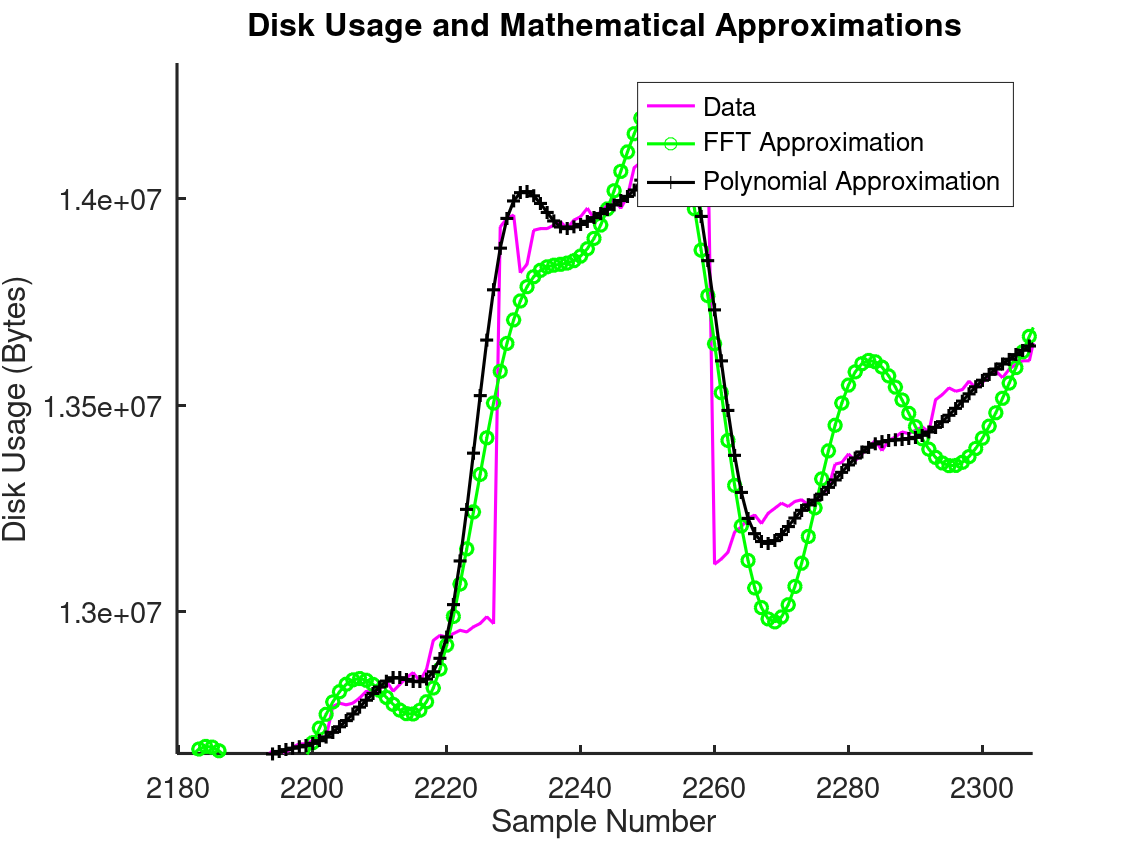
\includegraphics[width=0.5\textwidth]{math_approximation-3.png}
  \caption{A disk usage metric approximated by a Fast Fourier Transform and a Catmull-Rom interpolation.}
  \label{math_aprox}
\end{figure}

Prior to the mathematical modelling of the signal, the data is split into blocks with a dynamic size.
This is complemented by an indexing technique that allows the streaming of data without its complete decompression.
The compressor can either operate in lossy or lossless mode. Importantly, even when operating in a lossy manner, the information is preserved  .
The compression ratios achieved using our method enables avoiding data aggregation techniques and culminate in storage and compute savings.
% Give an overview of the paper’s structure
In the following sections, we discuss the context leading to our research while exploring the architecture of our compressor and providing a detailed explanation of its dynamic blocking, modelling, and indexing aspects. Furthermore, we expand on the topic of error correction for minimizing compression artifacts and discuss the results obtained with this approach on production datasets.

\section{Background}

In the dynamic landscape of computer systems monitoring, the impetus for our research stems from critical challenges that impact the efficiency and cost-effectiveness of current practices. 

\subsection{High Storage Cost}

The exponential growth of data in computer systems monitoring has led to soaring storage costs. Traditional methods often struggle to cope with the sheer volume of information generated by processes, databases, and overall system health monitoring. Our research delves into innovative time-series compression techniques that alleviate the burden of high storage costs, offering a sustainable solution for data retention and management. 

\subsection{Balancing Data Reduction and Information Preservation}
Conventional practices often resort to techniques such as averaging, sub-sampling or undersampling to manage the overwhelming data volumes. This approach effectivelly reduces the amount of data points but is undermined by the loss of valuable information . Our research addresses this trade-off by proposing advanced time-series compression methods that achieve data reduction without sacrificing critical insights and information. 

\subsection{Computational Challenges in Traditional Monitoring Techniques}
Traditional approaches, such as point-walking algorithms, demand substantial computational resources to process vast amounts of monitoring data. Recognizing the strain on computing capabilities, our method introduces a more resource-efficient paradigm by exploring novel compression techniques inspired by audio processing.

Our comprehensive approach tackles the immediate challenges of high storage and egress costs while addressing the inherent trade-offs of data reduction techniques. The overarching goal is to improve the landscape of computer systems monitoring by introducing a cost-effective and information-rich paradigm through advanced time-series compression.  

\section{Architecture}

In this section we describe the internals of the ATSC compressor. That includes both compressor\ref{internal} and decompressor, also internal structures and any other auxiliary mechanisms used.

\begin{figure}[h]
  \centering
  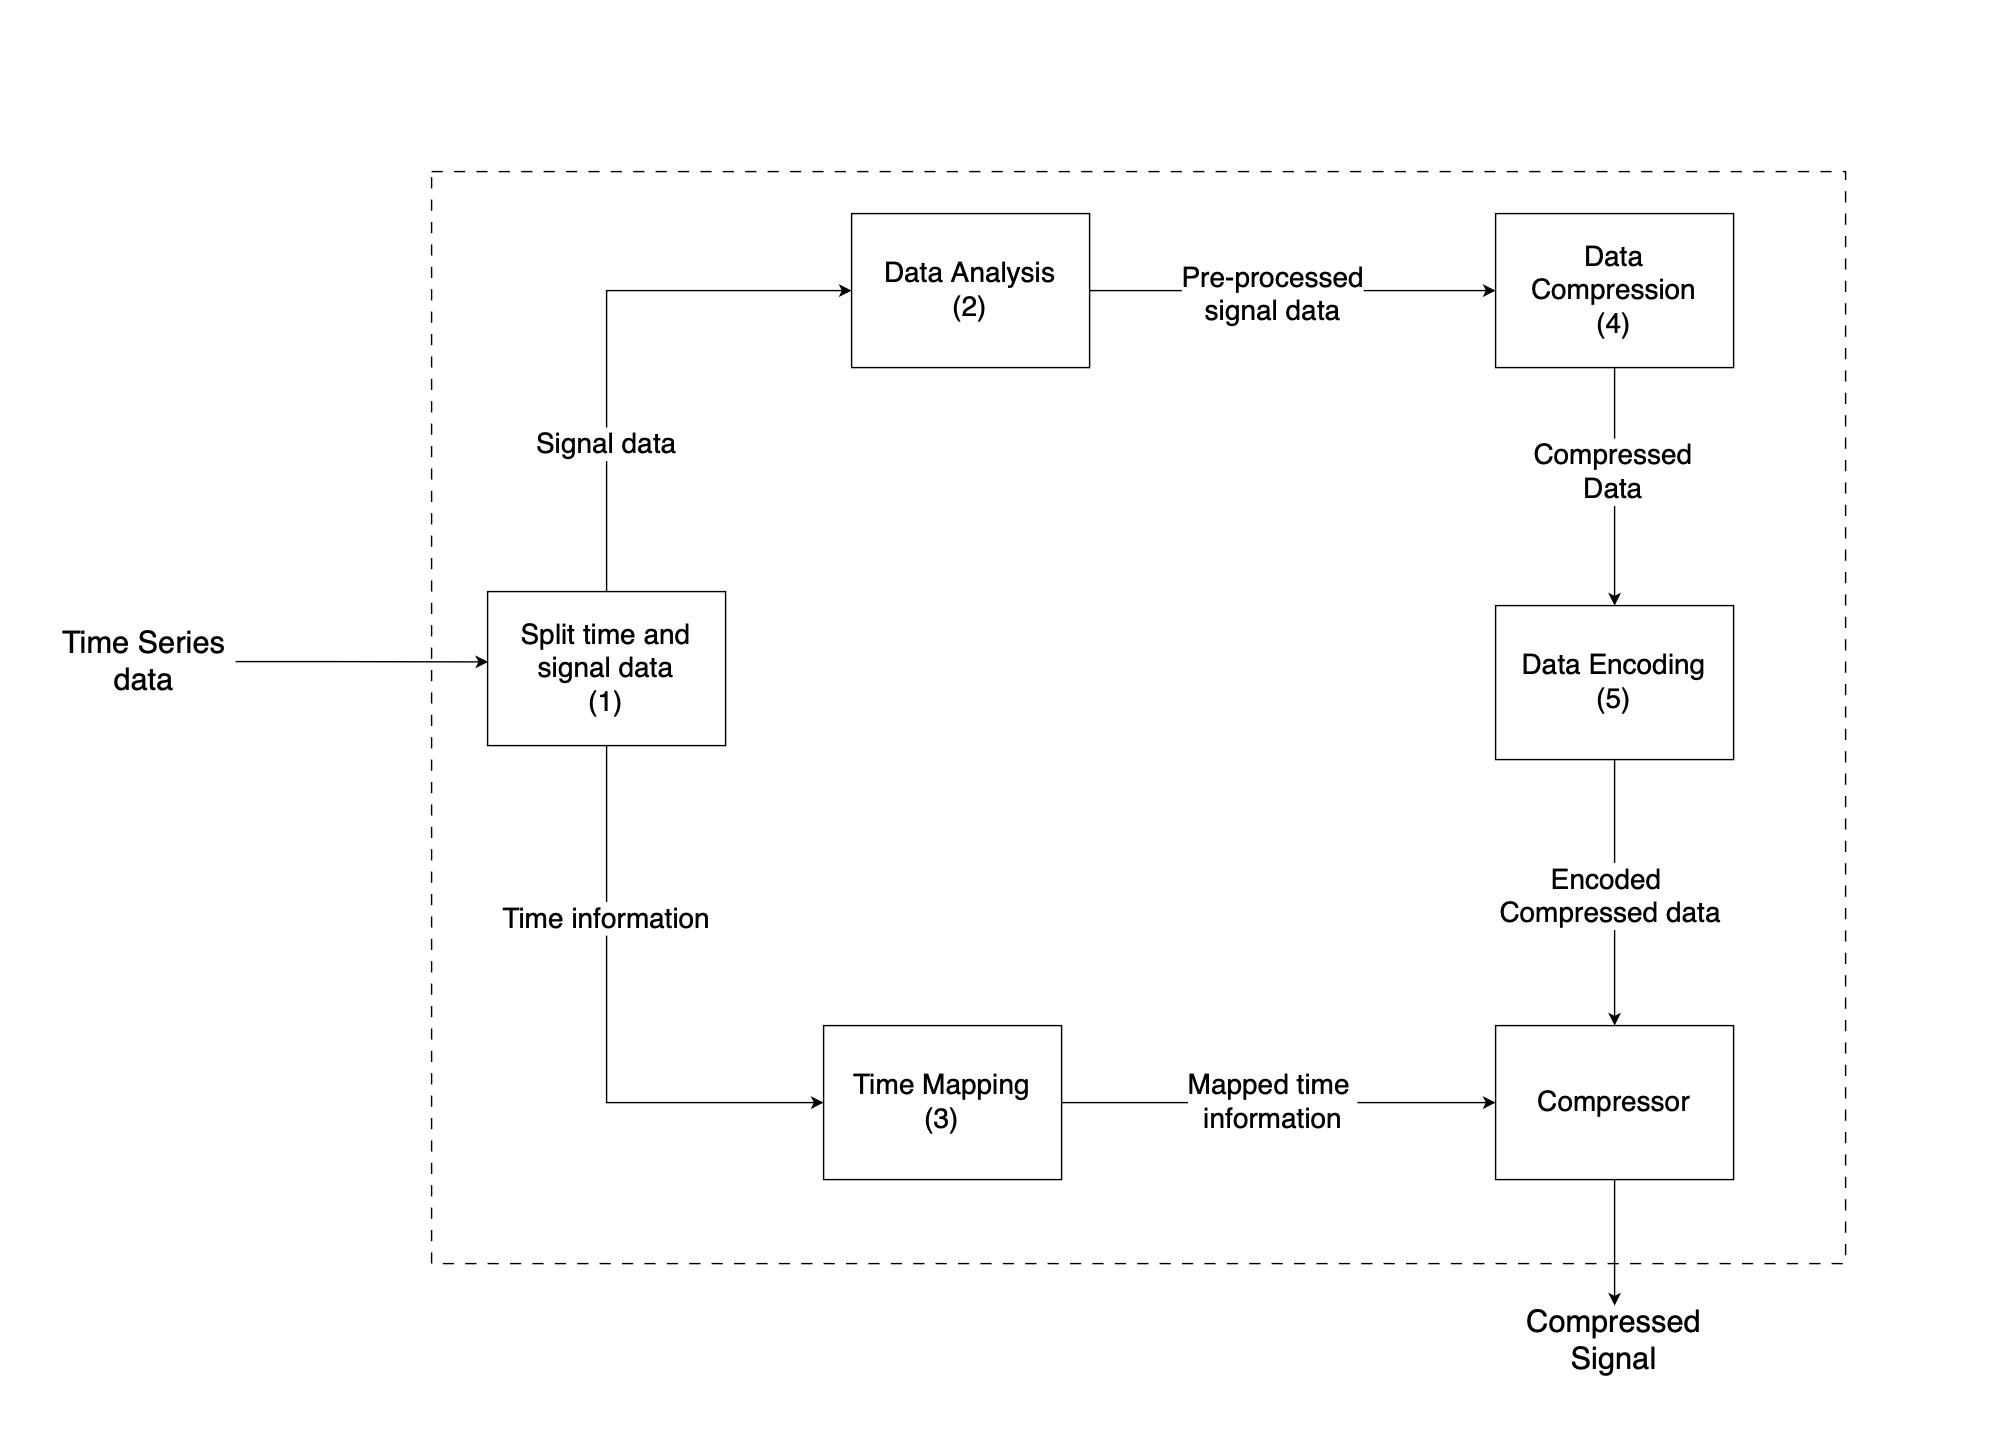
\includegraphics[width=0.5\textwidth]{Fig2.png}
  \caption{Internal Diagram of the ATSC Compressor stage}
  \label{internal}
\end{figure}

\subsection{ATSC Compressor}

\subsubsection{Split time and signal data}
First part of the processing is to split the signal into is two components, time and the signal.

\subsubsection{Data Analysis}
In this stage signal undergoes a statistical pre-processing, calculating the minimum, maximum, mean, variance, etc.
Also, the splitting of the signal into different blocks is performed here.
The block sizes are dynamic, and the sizing is done via 2 methods, either a discrete wavelet transform (DWT)\ref{wavelet} or sizing for optimal FFT processing (in the form of $slice = 2^n * 3^m$).
Given the computational cost of DWT, smaller signals are immediately sliced for FFT optimal size. In the other cases, DWT is performed first and if there is no high frequency components detected for slicing, FFT sizing is then performed.
This information is provided to the Data Compression stage along with the signal data.

\begin{figure}[ht]
  \centering
  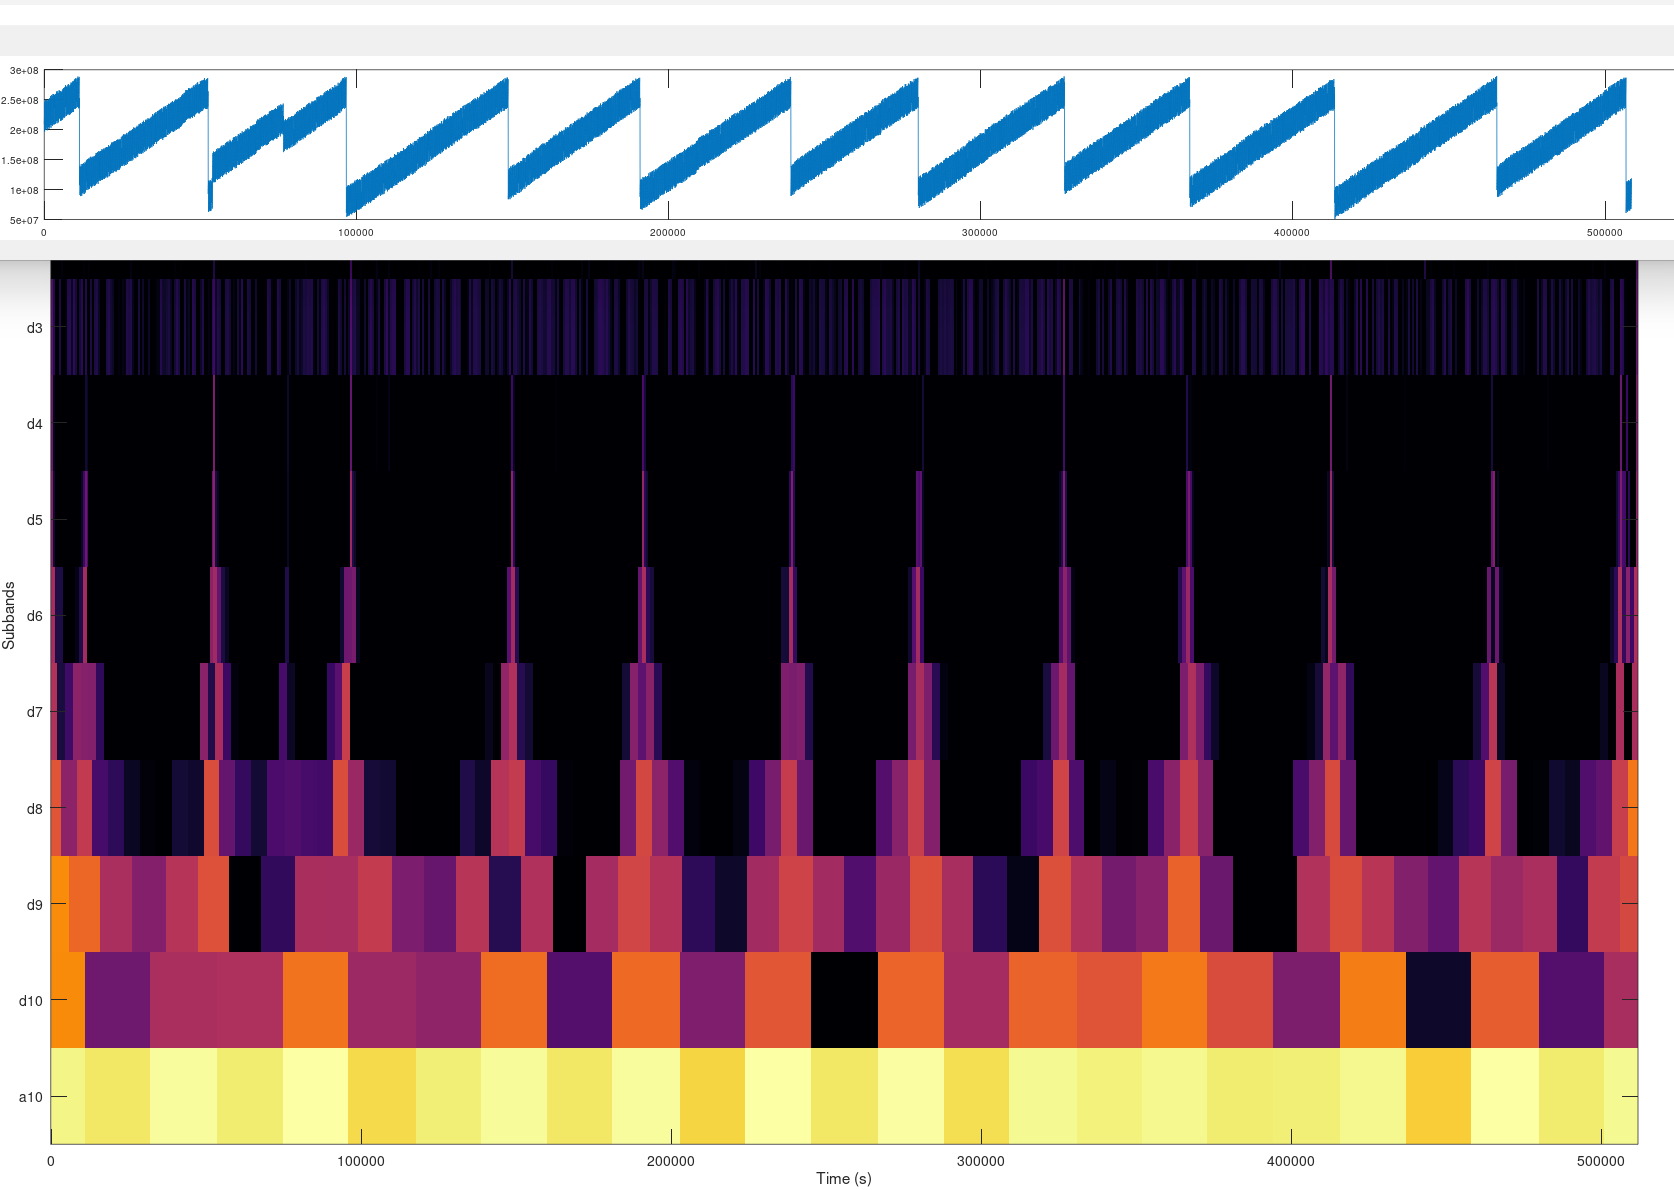
\includegraphics[width=0.5\textwidth]{wavelet_heap.png}
  \caption{Example of wavelet detection of high frequency sections to slice the signal. Signal on top and Wavelet Analysis on bottom.}
  \label{wavelet}
\end{figure}

\subsection{Time Mapping}
To facilitate precise access to samples without the need for full file seeking or decompression of the full file, ATSC generates a an index. This index ensures efficient retrieval of relevant portions of the signal, a critical aspect in the decompression and streaming processes.
The indexing technique is further explained in his own section.

\subsubsection{Data Compression}
The signal samples are divided into blocks, and for each block, ATSC applies modelling techniques tailored to the specific characteristics of the signal. 
This may involve techniques such as Linear Predictive Coding (LPC), Polynomial Prediction, Fast Fourier Transforms (FFT), or other methodologies that best suit the signal's behavior. 
For a special case of signals that are continuous only a single value is stored, alongside the number of samples.
This modeling converts the original samples into an approximated formula.
In some cases it is possible to match the original signal precisely and no other data is stored, otherwise an array of values representing the biggest outliers are stored alongside the formula type and its components.
This leads to a high number of data points being converted into a mathematical formula and its components.
Error correction and artifact reduction are also performed at this stage.
A deeper dive into this is done in the Compression\ref{section:compression} section of this study.

\subsubsection{Data Encoding}
The last step of optimization is done by reducing the information to the minimal computational size needed for each sample. 
Samples are normally provided in 64bits size, this step can reduce the sample size to 8bit or any other size that the samples fit.

\subsubsection{Compressor stage}
This is the final stage, it just joins the compressed data alongside the index.


\subsection{ATSC Decompressor}

ATSC distinguishes itself by eschewing the storage of timestamp information directly within the file, opting instead for a distinctive indexing approach that enables efficient streaming and targeted decompression of pertinent data segments.
Within the Read Path of ATSC, the samples are located via an indexing table, and then uncompressed, or the full content if requested. 
Since speed is important in retrieval of metrics, the read stage, after the location of the samples, applies the mathematical formula defined for the sample segment plus any error correction, and the returns the samples. 

\subsubsection{Precise Streaming through Specialized Indexing}\label{SCMA}
The core innovation in the Read Path lies in the application of a specialized indexing mechanism. Unlike traditional methods, ATSC's indexing facilitates pinpointing the relevant portion of the file without the necessity of timestamp inclusion in the file itself. This precision in indexing empowers ATSC to streamline the streaming process, focusing exclusively on the required data, thereby optimizing resource utilization. 

\subsubsection{Decompression process}

\begin{itemize}
\item{\textbf{\textit{Identifying the Samples to be Retrieved:}}} The Read Path initiation begins with the user specifying time interval of metric of interest. If no interval is provided, all samples are returned.
\item{\textbf{\textit{Data Retrieval Using the Index:}}} The index plays a crucial role in ATSC's approach. It aids in precisely identifying the segment of the file essential for the query. This ensures focused and efficient data retrieval.
\item{\textbf{\textit{Sample decompression:}}} Once the relevant data segment is identified, ATSC initiates the decompression of the data.
For the located data samples, the correspondent formula translation is applied and any error correction.
\item{\textbf{\textit{Timestamp Integration Post-Decompression:}}} Following decompression, the samples, now in their extracted form, receive timestamp information from the index. This final step ensures temporal accuracy and relevance of the retrieved data.
\item{\textbf{\textit{Streaming/Writing data out:}}} Under a streaming process, samples are sent while being decompressed. ATSC also supports full file decompression where all the data is decompressed and then send out, or written out to a WAVBRO file.
\end{itemize}

\section{Compression Methods}\label{section:compression}

Most of the work is done in this step. 
After a statistical analysis the signal, the compressor stage decides which approach is best for a given block of samples.
Things like first and second derivative analysis also allows a more precise selection of the compression form. 
For example, a signal which is mostly stable (small variation) will be approximated by a Spline, a signal with a lot of variation will be better approximated by an Fast Fourier Transform or Linear Predictive Coding.
Depending on the error allowed for the compression, a less optimal method might be selected trading off precision for space savings. 

\vspace{10pt}
\subsubsection{Fast Fourier Transforms (FFT)}

Compression with FFT is done via a conversion of the signal to the frequency domain. Once in the frequency domain, we store a subset of frequencies.
The number of frequencies selected depends on the error margin we want to store the signal with. Since the signals are always real, the worst case scenario (lossless compression) half the frequencies need to be stored.
But since every frequency is represented by a pair of (Real, Imaginary) values, the lossless compression is next to none. 
The frequency pairs are always represented by two floats, either 32 or 64 bits depending on the precision required.
In a lossy scenario, and depending on the signal, 10x reduction in size is easily achievable within a 1\% to 3\% error margin.
To decompress, the Inverse FFT is applied on the available frequencies, zeroing out the missing frequencies.

\begin{figure}[ht]
  \centering
  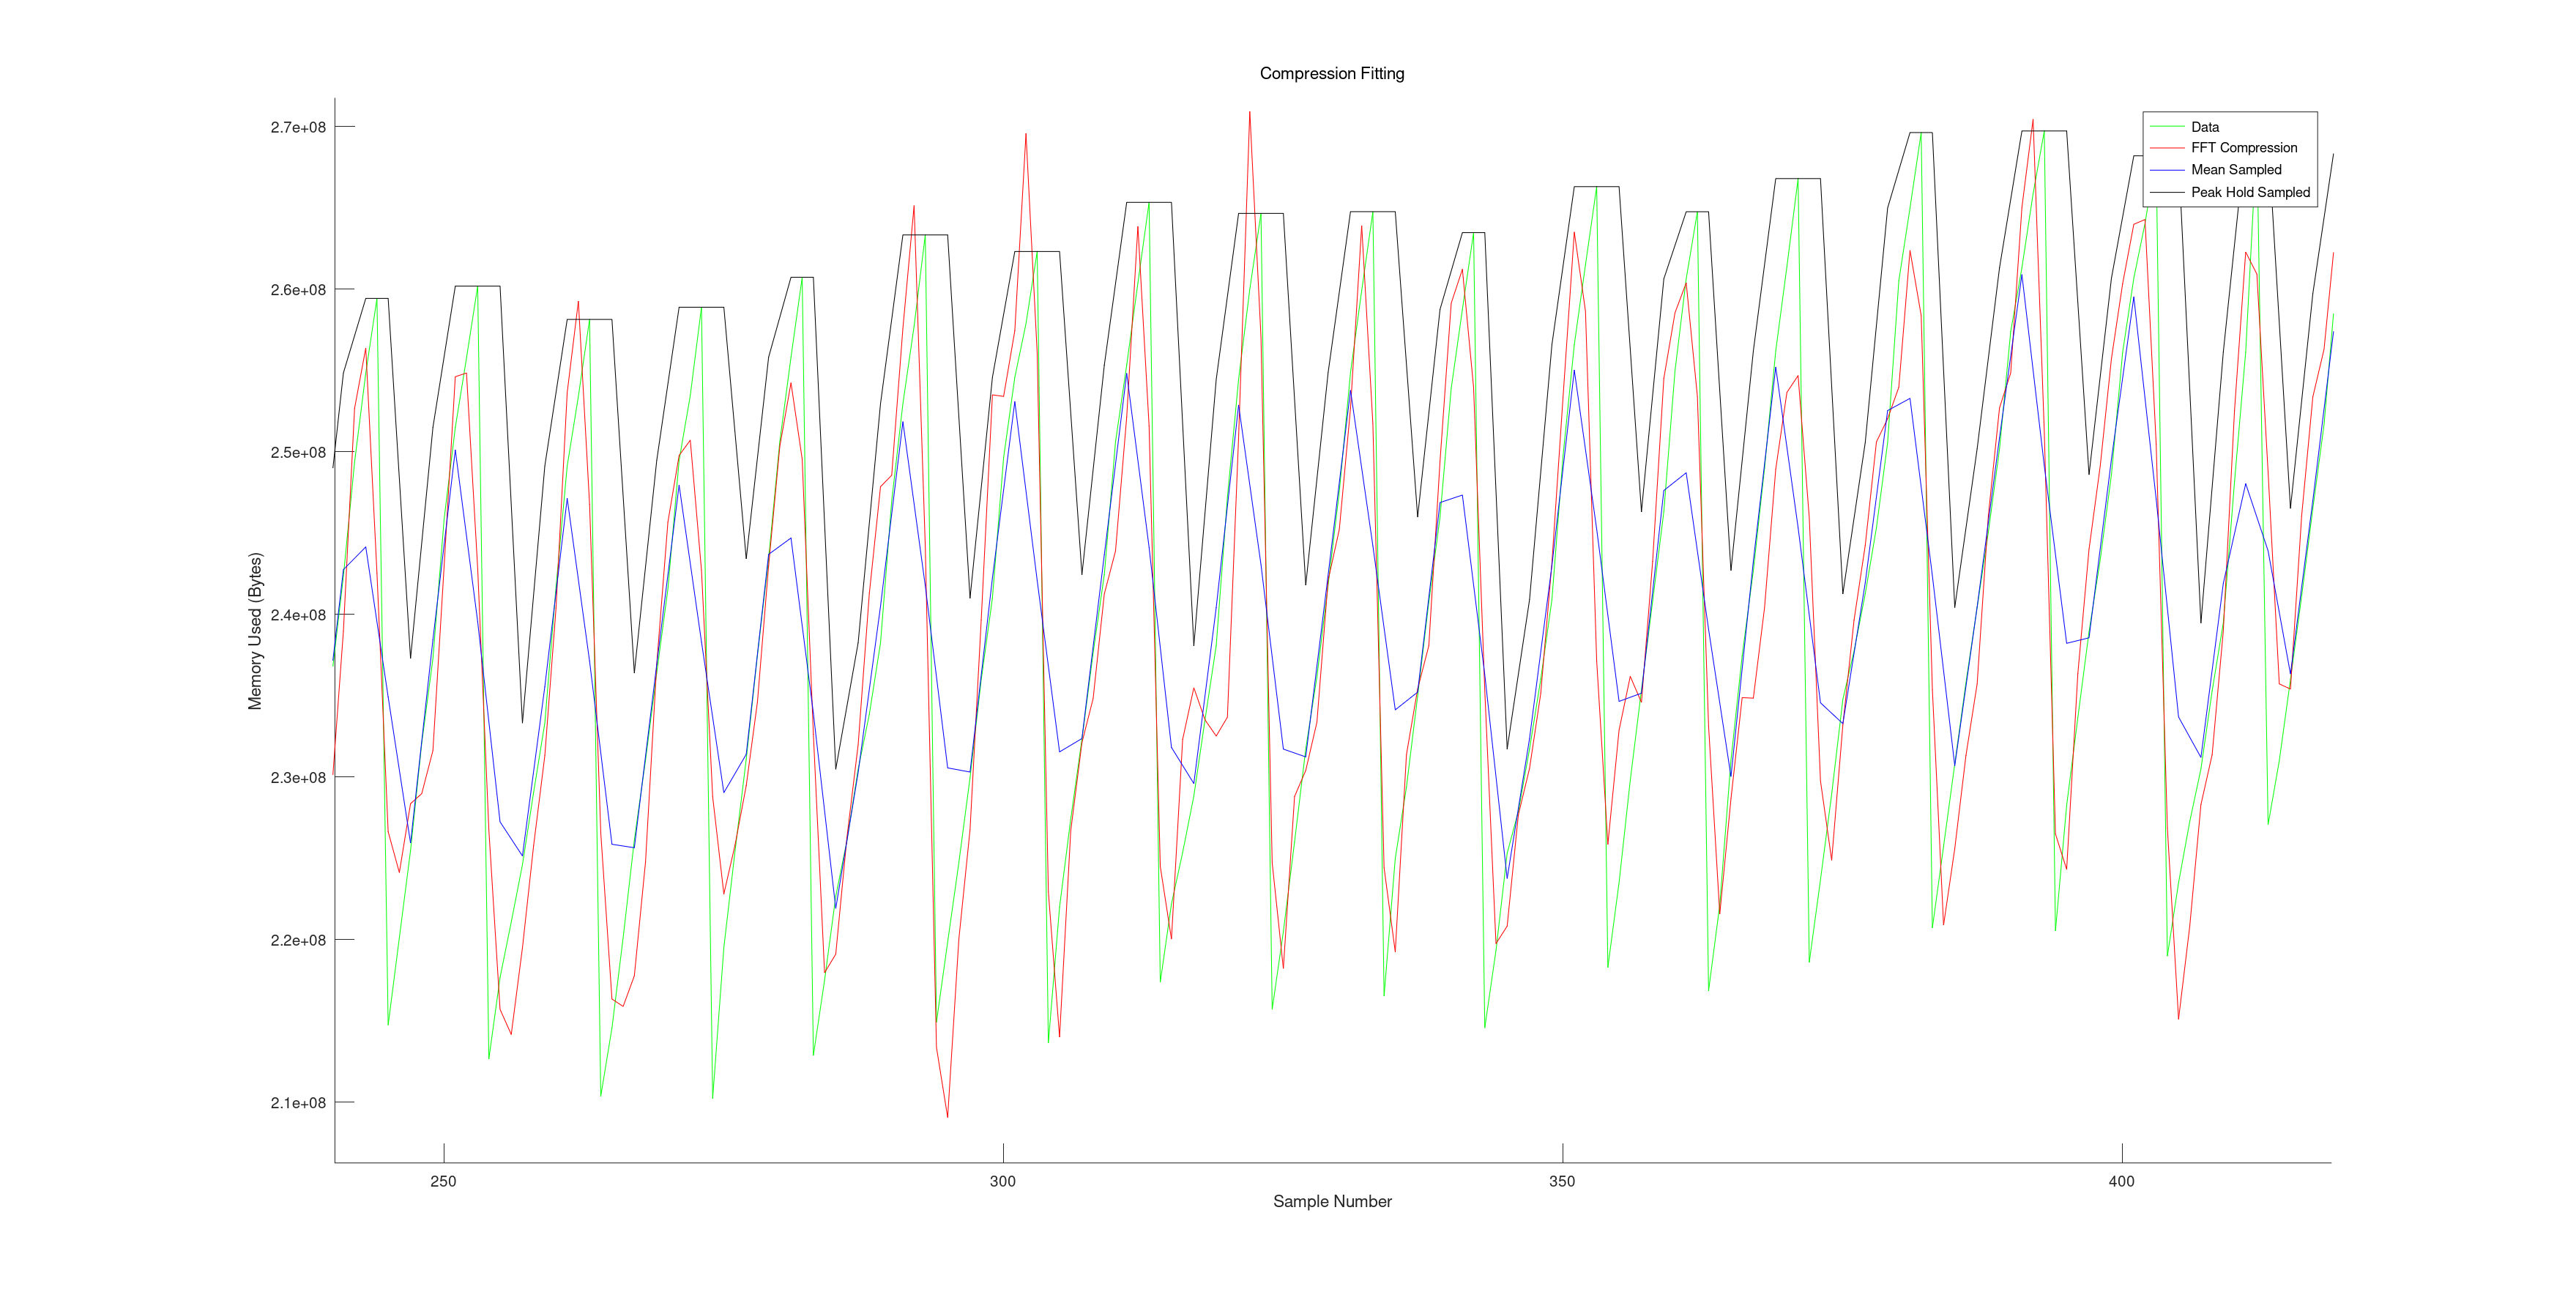
\includegraphics[width=0.5\textwidth]{FFT_Comparison.png}
  \caption{Signal Fitting of the original data vs FFT Compression (8x compression) vs Average Sampled (2x) and Peak Hold (2x).}
  \label{fft_comparison}
\end{figure}
\vspace{5pt}

\subsubsection{Spline Interpolation}

Another compression method is via a Spline Interpolation. Currently, using either linear for simple signals (near-linear signals like Disk usage) or Catmull-Rom interpolation for everything else.
The method is similar to the FFT, where several points are stored, and the corresponding outputs calculated via Spline Interpolation.
Once a Spline is generated within the margin of error provided, the points that generated that spline are stored.
An advantage of Spline Interpolation vs FFT is that the FFT always need to store the data as a pair of floats. 
While the Spline Interpolation the points are the same as the data points, so a integer signal would be stored as integer with the same bit depth as the original signal.
This could be something as small as 8bit per point.
In the decompression process, we do the interpolation calculation and retrieve the points requested.
No need even to calculate the whole spline, only the segments corresponding to the samples.

\vspace{10pt}
\subsubsection{Multivariate Interpolation}

In an almost identical process to the Spline Interpolation, we used Inverse Distance Weighting as a method to approximate the signal.
The results are solid, but almost the same as the spline interpolation, with the downside of a much slower decompression due to the complexity of the calculations.
Since the approach is very similar, the results were very easy to compare, and in most of the cases the Spline Interpolation offers the same compression this method is used
only in very rare cases.
The similarity of the two also makes it difficult to choose each one to pick in a given scenario, and given the already mentioned disadvantages, this is only used in a manual selection of compressor methods.

\begin{figure}[ht]
  \centering
  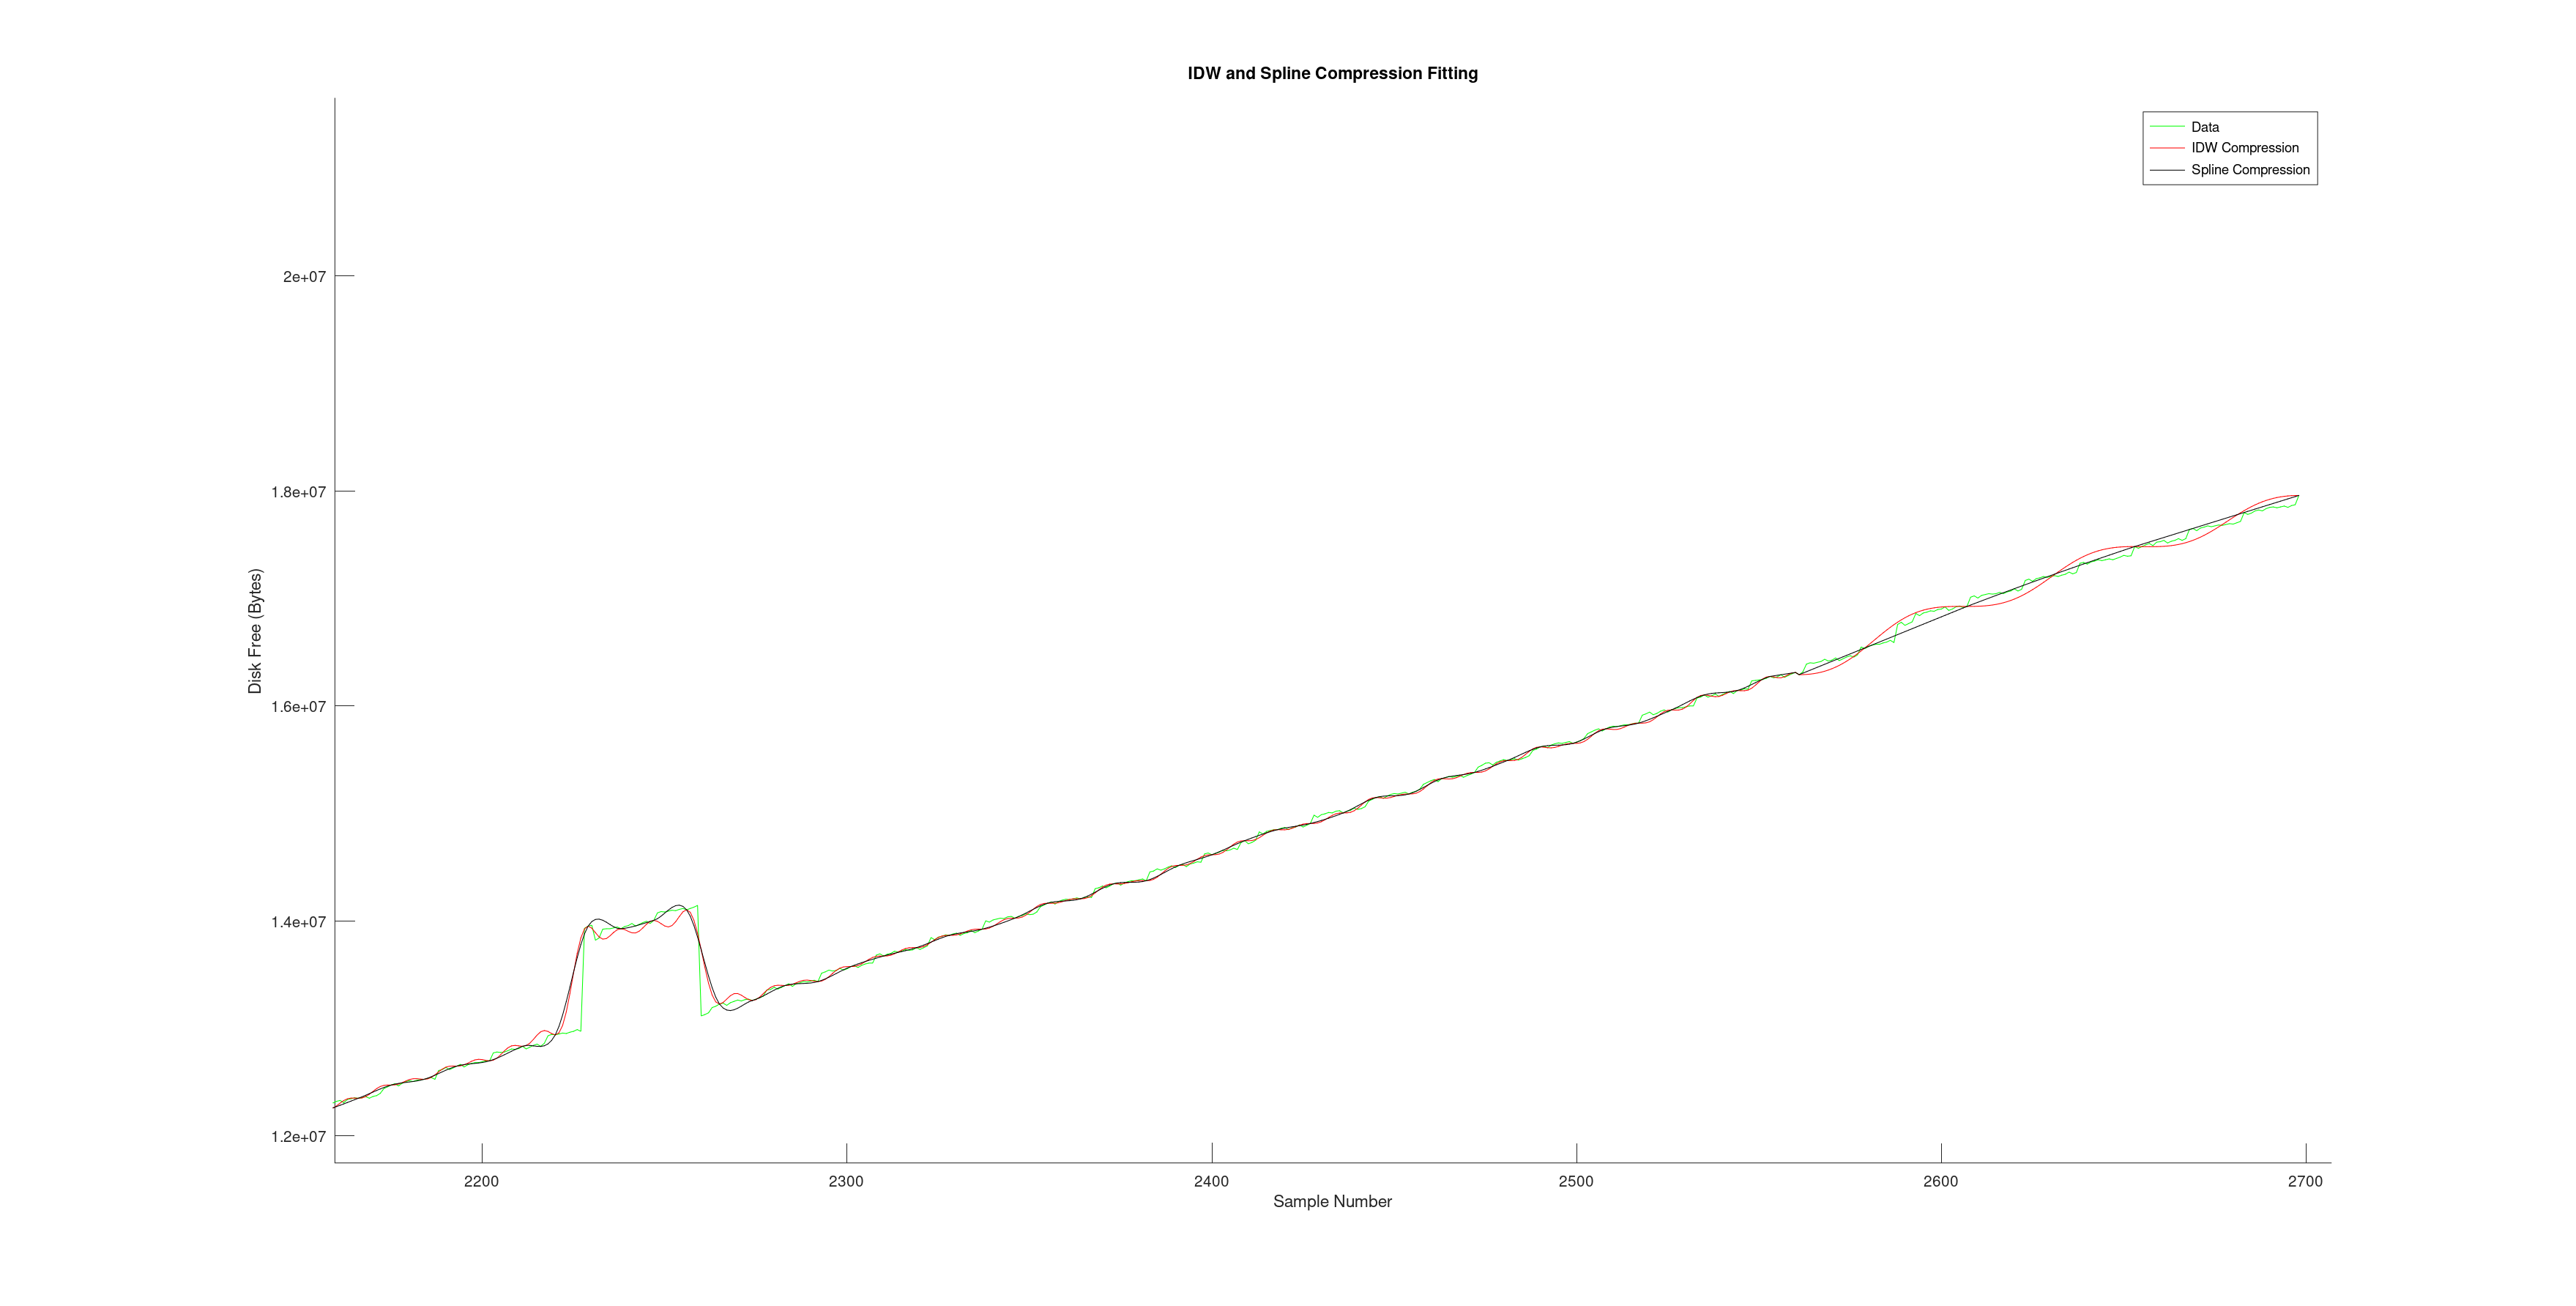
\includegraphics[width=0.5\textwidth]{IDW_Spline_Comparison.png}
  \caption{Signal Fitting of the original data with IDW Compression and Spline Compression (Both 43x compression).}
  \label{Fig.4}
\end{figure}
\vspace{5pt}

\vspace{10pt}
\subsubsection{Linear predictive coding (LPC)}

A lot of lessons were learned from initial experiments with Audio compressors (mostly FLAC encoder).
Good results were obtained, and it was a natural approach to include the those within the available compressors.
The approach is exactly the same as described in the FLAC format [11], but with a small change.
The FLAC expects all samples to be integer, as such, floating point signals are discarded and not usable by definition.
But for signals with a very small precision and bounded (e.g. 0.00 - 100.00) we can convert those to integer and use the LPC compressor.
In practical testing, LPC offers the worst compression, worse than FFTs, so FFT is widely used, and in a similar case as the Inverse Distance Weighting, it is mostly relegated to a manual selection.
The only case where LPC is used, is in lossless compression, where it offers a very solid compression averaging between 4x to 8x.

\vspace{10pt}
\section{Artifact Detection and Correction}

All the methods described above generate almost always, a lossy compression. 
This is as expected since is the core part of our work. 
But sometimes, the methods above might generate artifacts that we need to remove. 
Those artifacts are points that are generated from the mathematical approximations and are far from the original data points.
They constitute point errors bigger than any other points in the generated data.

\begin{figure}[ht]
  \centering
  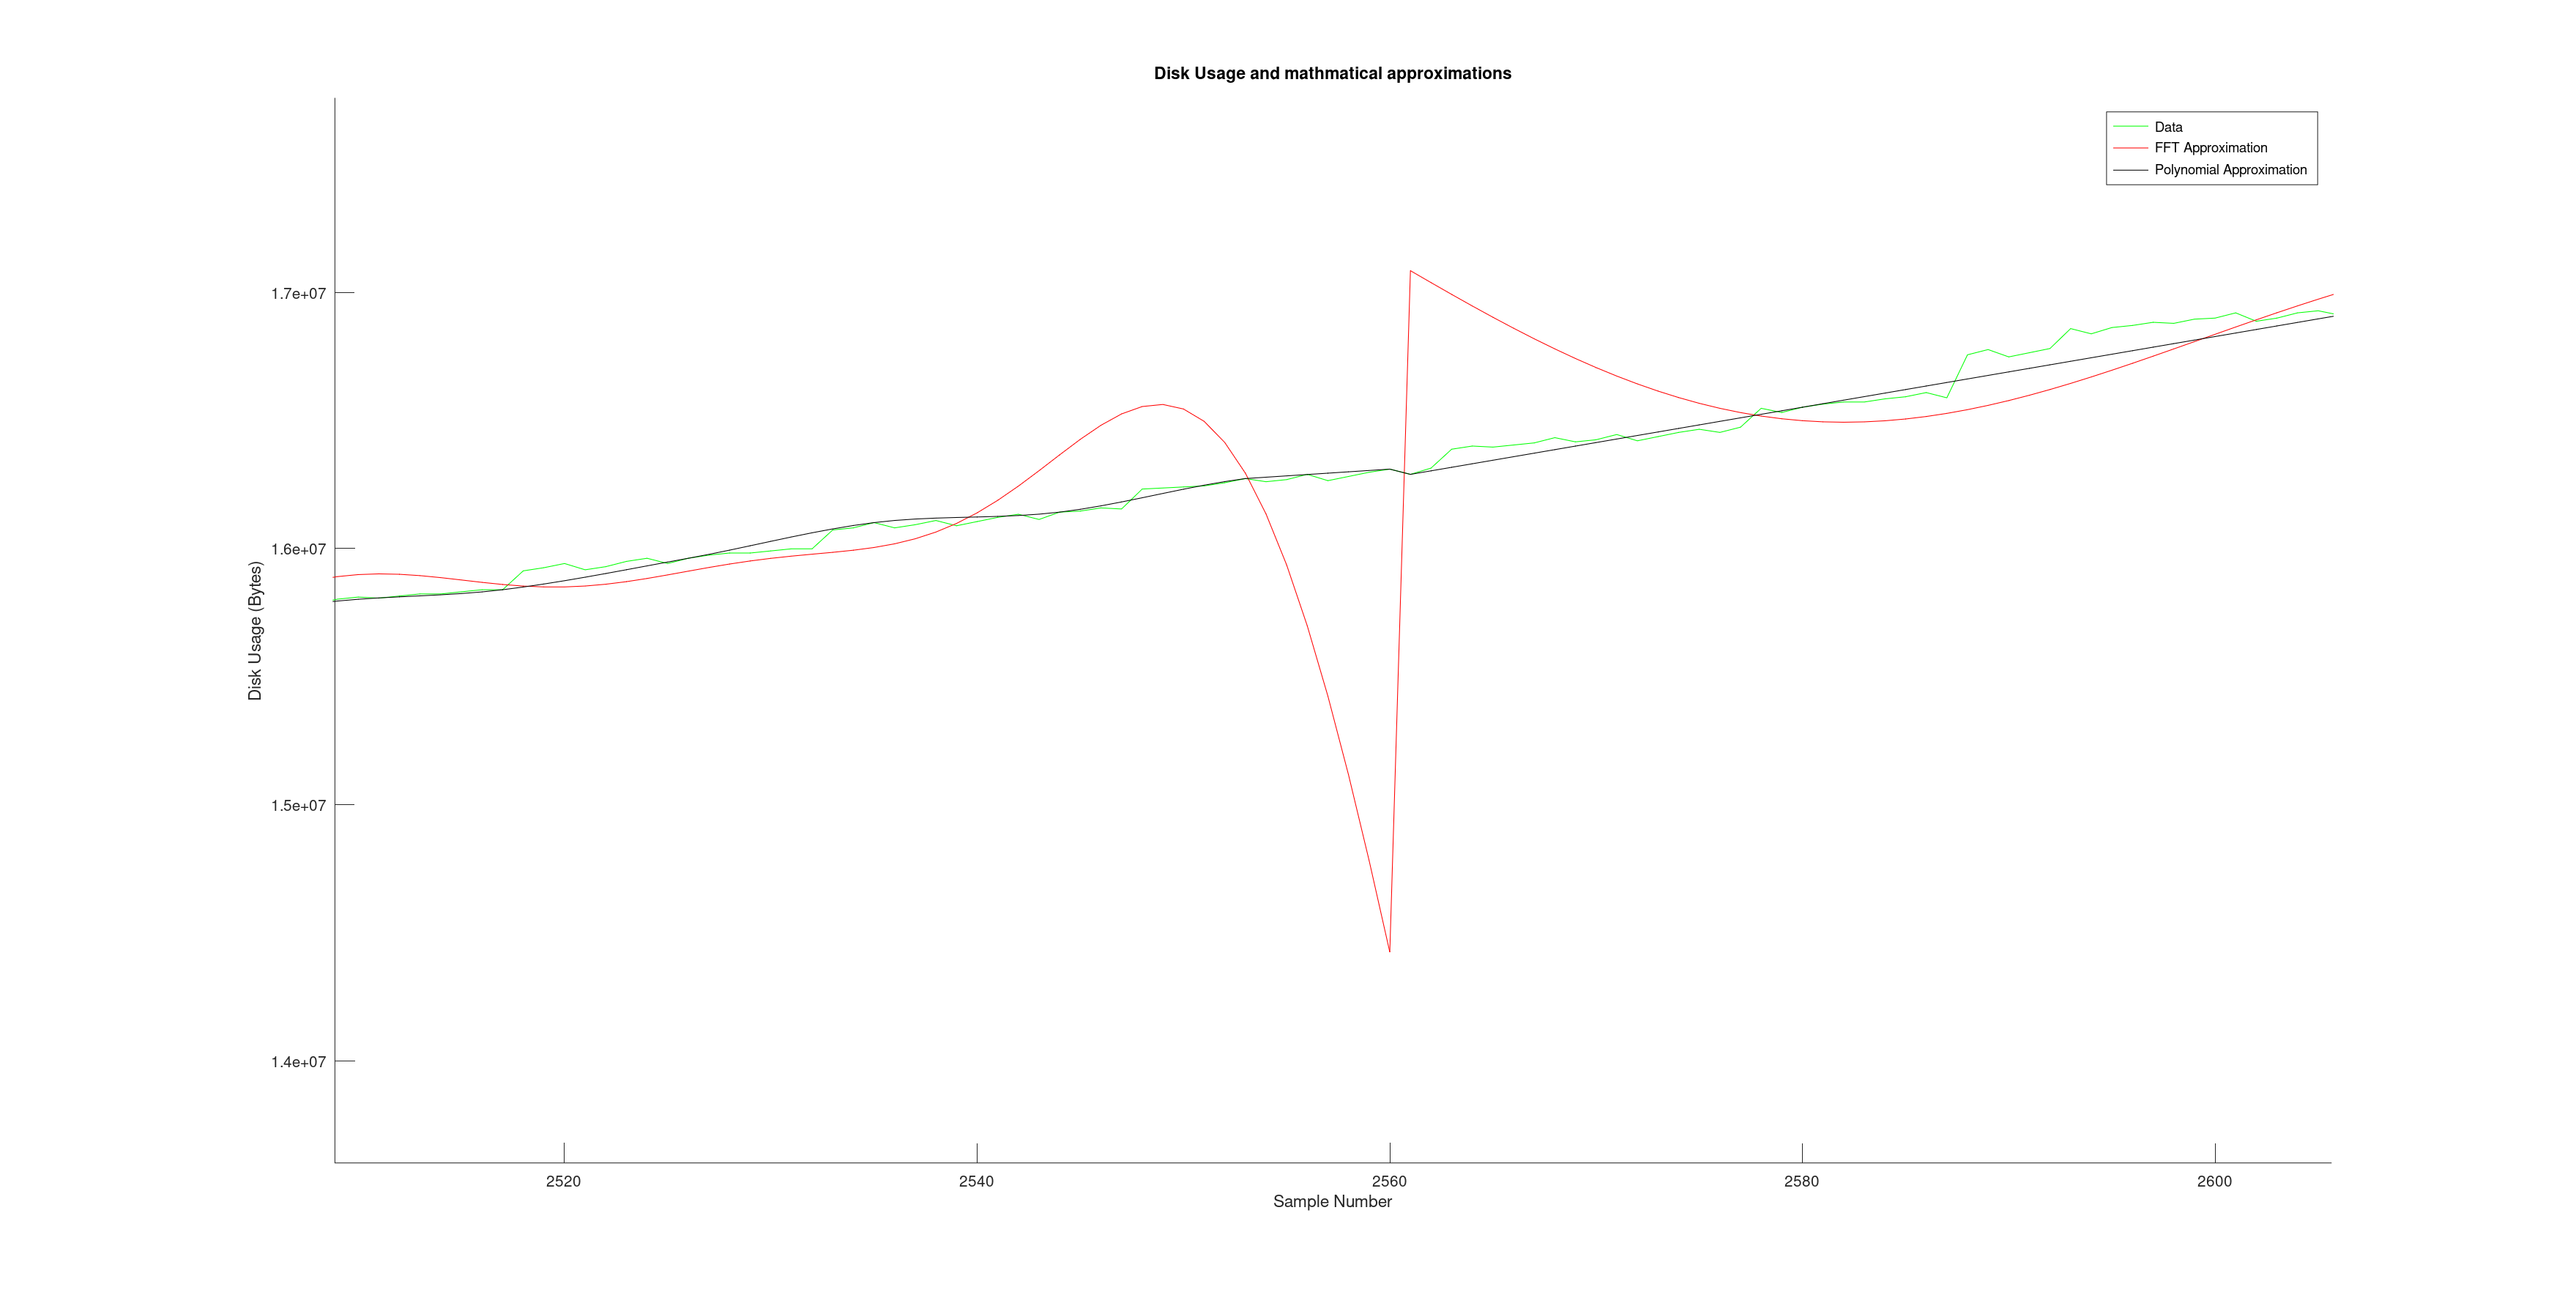
\includegraphics[width=0.5\textwidth]{compression_artifact.png}
  \caption{Compression artifact from the FFT approximation.}
  \label{fig:artifact}
\end{figure}
\vspace{5pt}

For reducing the error of the compression and/or remove artifacts from the generated signals the following process is used:

\begin{itemize}
    \item Error detection via Mean Absolute Percentage;
    \item Storing of the errors that are above the defined error threshold;
    \item Store the location of the biggest errors and the correspondent original data point;
    \item When decompression happens, replace the generated points by the stored data.
\end{itemize}

This approach not only removes the biggest artifacts from the data, it also lowers the error rate of the signal. On a good fitting, we can avoid storing any point, so the importance of the fitting.
A tradeoff exists, since getter a better fitting need more data stored (e.g. More frequencies for FFT), and storing errors need space. But even a good fitting, needs artifacts removed.
For lossless compression all the point differences need to be stored.
In a lot of cases this leads to almost no compression unless the signal has a perfect fitting with the mathematical representation.

\section{Indexing Samples with VRSI (Variable Rate Sampling Interval)}
\vspace{5pt}
\subsubsection{Overview of VRSI Mechanism}

In the methodology section, a critical aspect of the process involves indexing samples for efficient data retrieval. Variable Rate Sampling Interval (VRSI) is employed to manage the sampling intervals effectively. VRSI operates on the premise that samples occur at evenly spaced intervals, such as every 5 seconds, 20 seconds, or 60 seconds.
\vspace{5pt}
\subsubsection{Line Segment Representation}

For each sampling interval, a line segment is created with specific fields:

\begin{itemize}
    \item \textbf{Start Timestamp:} The timestamp marking the beginning of the sampling interval.
    \item \textbf{Sample Interval:} The time gap between consecutive samples.
    \item \textbf{Starting Sample:} The index of the first sample within the segment.
    \item \textbf{Number of Samples:} The total number of samples within the segment.
\end{itemize}
\vspace{5pt}
\subsubsection{File Structure}

These line segments are then stored in a file, accompanied by the lowest and highest timestamps in the segments represented. This file structure allows for easy identification of whether a requested interval is present in the index. If the requested interval falls entirely outside the timestamps in the file header, no samples are available for that interval.
\vspace{5pt}
\subsubsection{Handling Temporal Gaps}

In cases where a metric stops reporting for a period, a new line segment is generated, ensuring accurate representation of the sampled data over time.
\vspace{5pt}
\subsubsection{Example VRSI File Content}

\begin{verbatim}
55745
59435
15,0,55745,166
15,166,58505,63
\end{verbatim}


\begin{itemize}
    \item Line 1) Represents the first timestamp.
    \item Line 2) Represents the last timestamp.
    \item Line segments are detailed below:
    \begin{itemize}
        \item The first line segment has one sample every 15 seconds, starting at timestamp 55745, with a total of 166 samples.
        \item The second line segment also has one sample every 15 seconds, starting at timestamp 58505, with 63 samples.
    \end{itemize}
\end{itemize}
\vspace{5pt}
\subsubsection{Locating Samples (Read Path)}

In the read path, when locating a sample in a file using the index, timestamps or timestamp ranges are specified (e.g., "All the samples from 3:30 PM to 4:30 PM"). The system checks if the requested timestamps are within the available timestamps in the file header. If found, the sequence of sample numbers is extracted, indicating the samples needed for decompression.
\vspace{5pt}
\subsubsection{Creating/Updating the Index (Write Path)}

When a new sample is added, the index is updated. Since time progresses linearly, and samples occur in sequence, the system only needs to:
\begin{itemize}
    \item Update the last segment's sample number or
    \item Create a new segment.
\end{itemize}

Existing segments are incremented if the sample timestamp is the next in sequence. If a segment does not exist or the timestamp is not the next in sequence for the latest segment, a new segment is created. This approach ensures an efficient and organized index for managing variable rate sampling intervals.

% \begin{figure}[h]
%   \centering
%   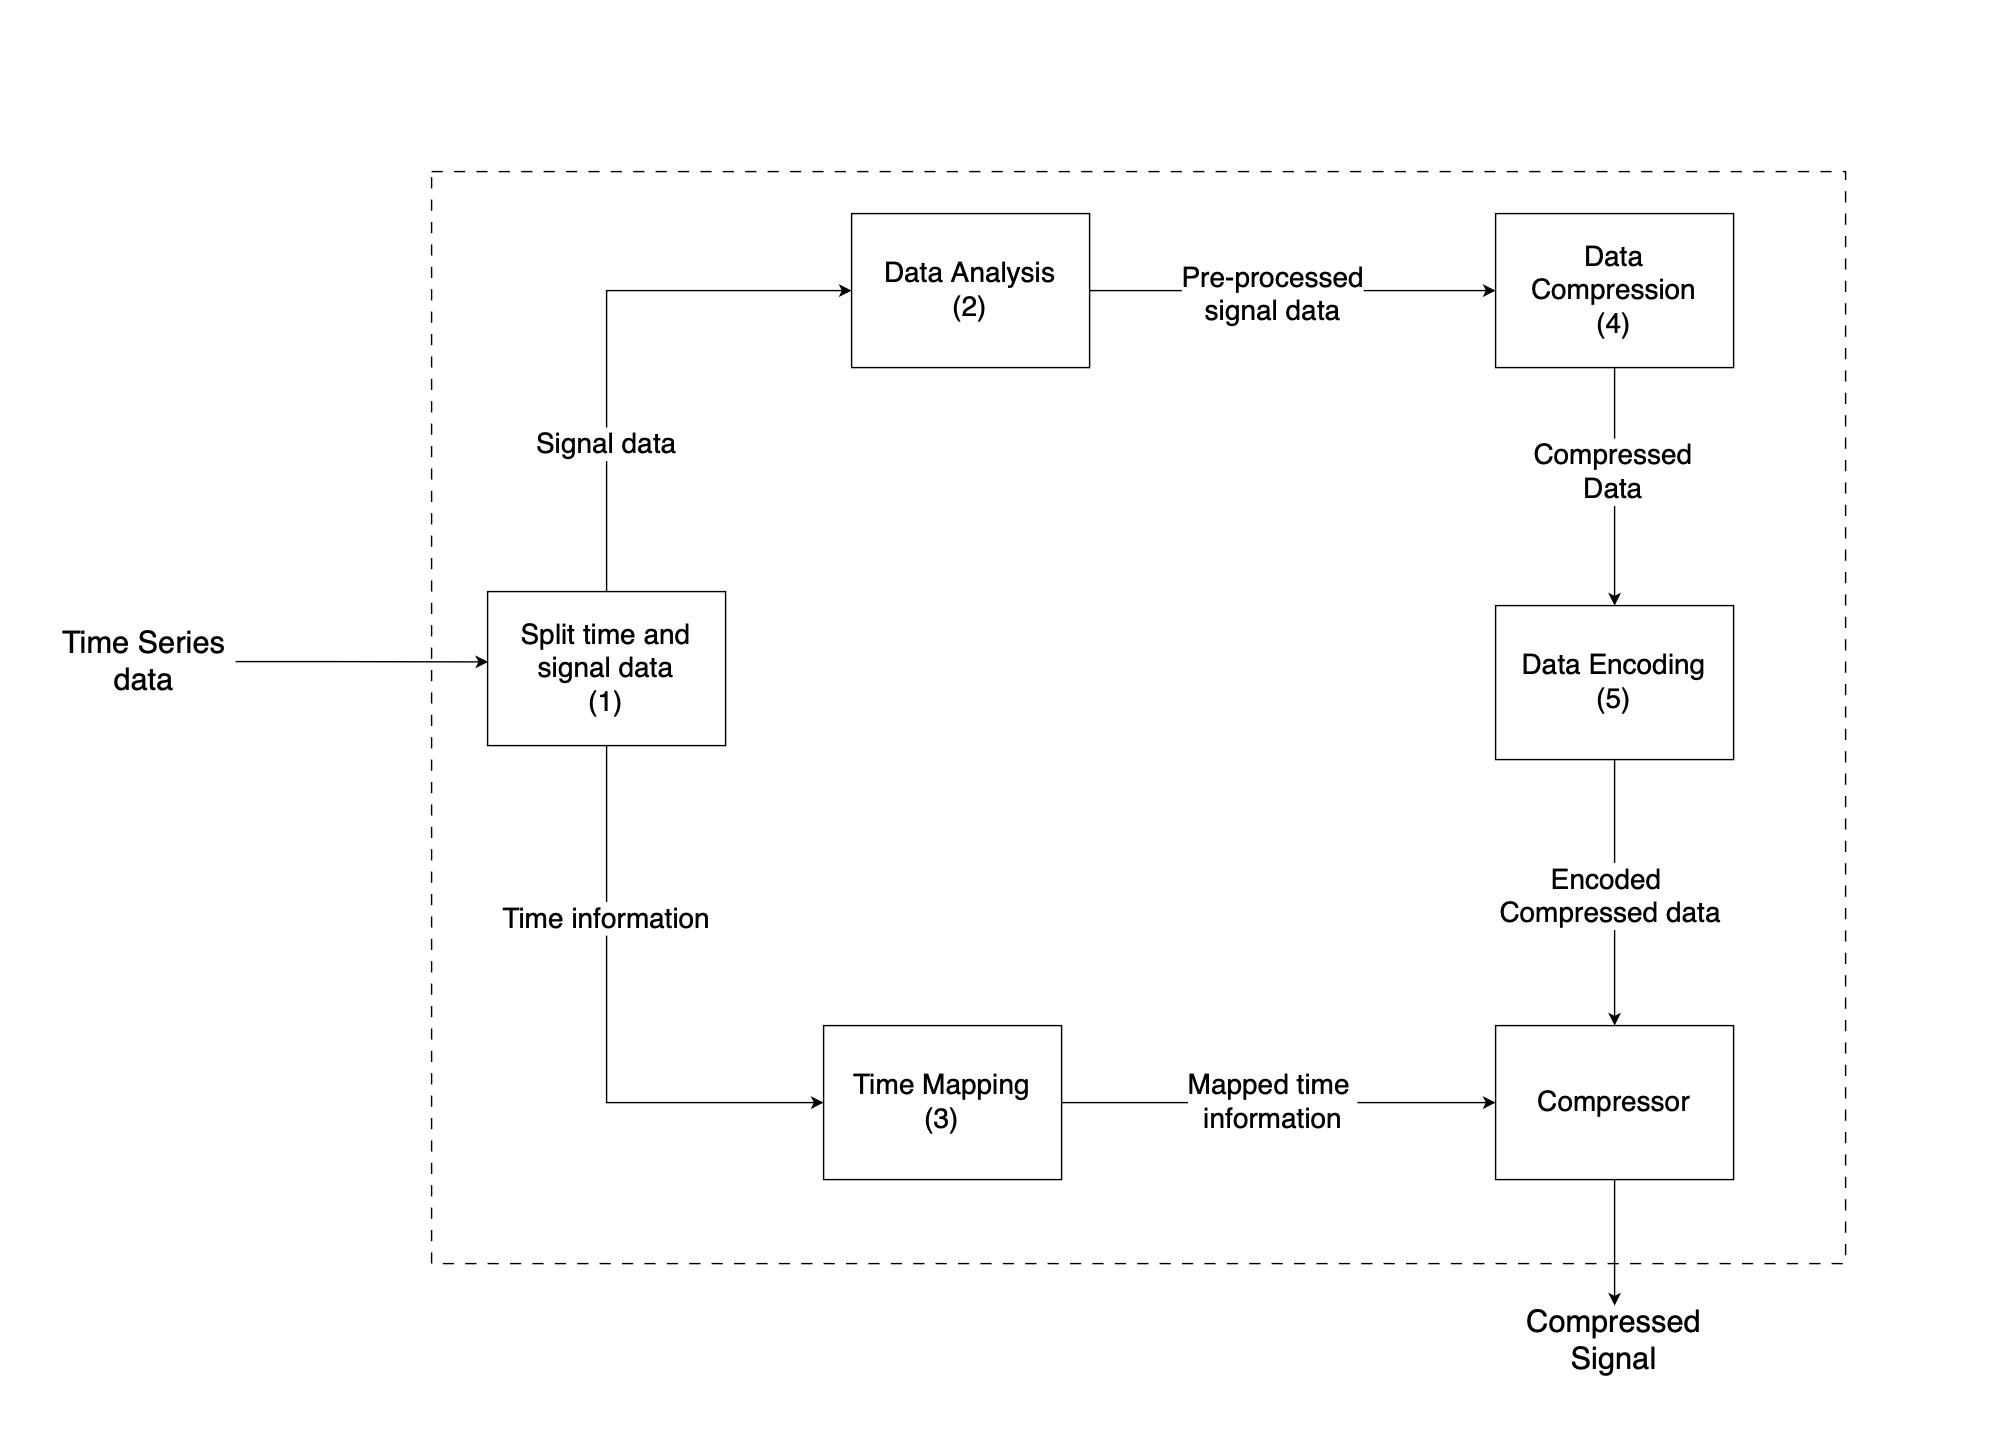
\includegraphics[width=0.5\textwidth]{Fig4.png}
%   \caption{Internal Diagram of the ATSC Compressor.}
%   \label{Fig.5}
% \end{figure}

\section{Results}

In our quest to assess the efficiency and effectiveness of ATSC, a comprehensive testing methodology was employed. 
The ATSC server was configured as both a read and write backend for a Prometheus instance, establishing a practical and relevant testing environment. 
This Prometheus instance, in turn, was connected to an Instaclustr internal production 57-node Cassandra cluster with a Prometheus endpoint enabled. 
The data flow was then collected at the node level, sent to Prometheus endpoint that would then forward it to the ATSC server configured as previously stated.
The server run for approximated 18h over 2 days. Collecting 1 point every 20 sec. This ended with 5432 samples for each signal, for each node.
A total of 14,386 signals processed.
Of this dataset, X are signals that represent aggregations (e.g. Histograms), so we removed those, and ended with 13,950 Signals.
ATSC run with automatic compressor selection and a maximum allowed error of 3\%.

\subsection{ATSC Single: A Best-Case Scenario Analysis}

Before delving into the detailed results, it is essential to address the ATSC single scenario.
The best case scenario for ATSC is a dataset that fits perfectly with a mathematical model.
In such a case, even with a growing number of samples it is possible to store a massive amount of data represented by only the mathematical formula, the sample number, and the index.
In such circumstances it is possible to achieve compression ratios of over 3000x.
One can question if this is a realistic scenario, and we answer: yes! As shown in our data overview, there are always signals that are stale, or change very infrequently, those fall in our best case scenario.
In our production testing, approximate 13\% of the data falls into the best case scenario.

\subsection{Data Overview}

\textbf{Raw Data Size:} 847,315,029 bytes \\
\textbf{Compression Statistics:}

\begin{table}
\centering
\begin{tblr}{
  hline{2} = {-}{},
}
\textbf{Module} & \textbf{Compressed size (bytes)} & \textbf{Compression Ratio}   \\
Prometheus                  & 454,778,552                      & 1.86 \\
LZ4                         & 141,347,821                      & 5.99 \\
ATSC                        & 14,276,544                       & 59.35                                    
\end{tblr}
\end{table}

\begin{figure}[h]
  \centering
  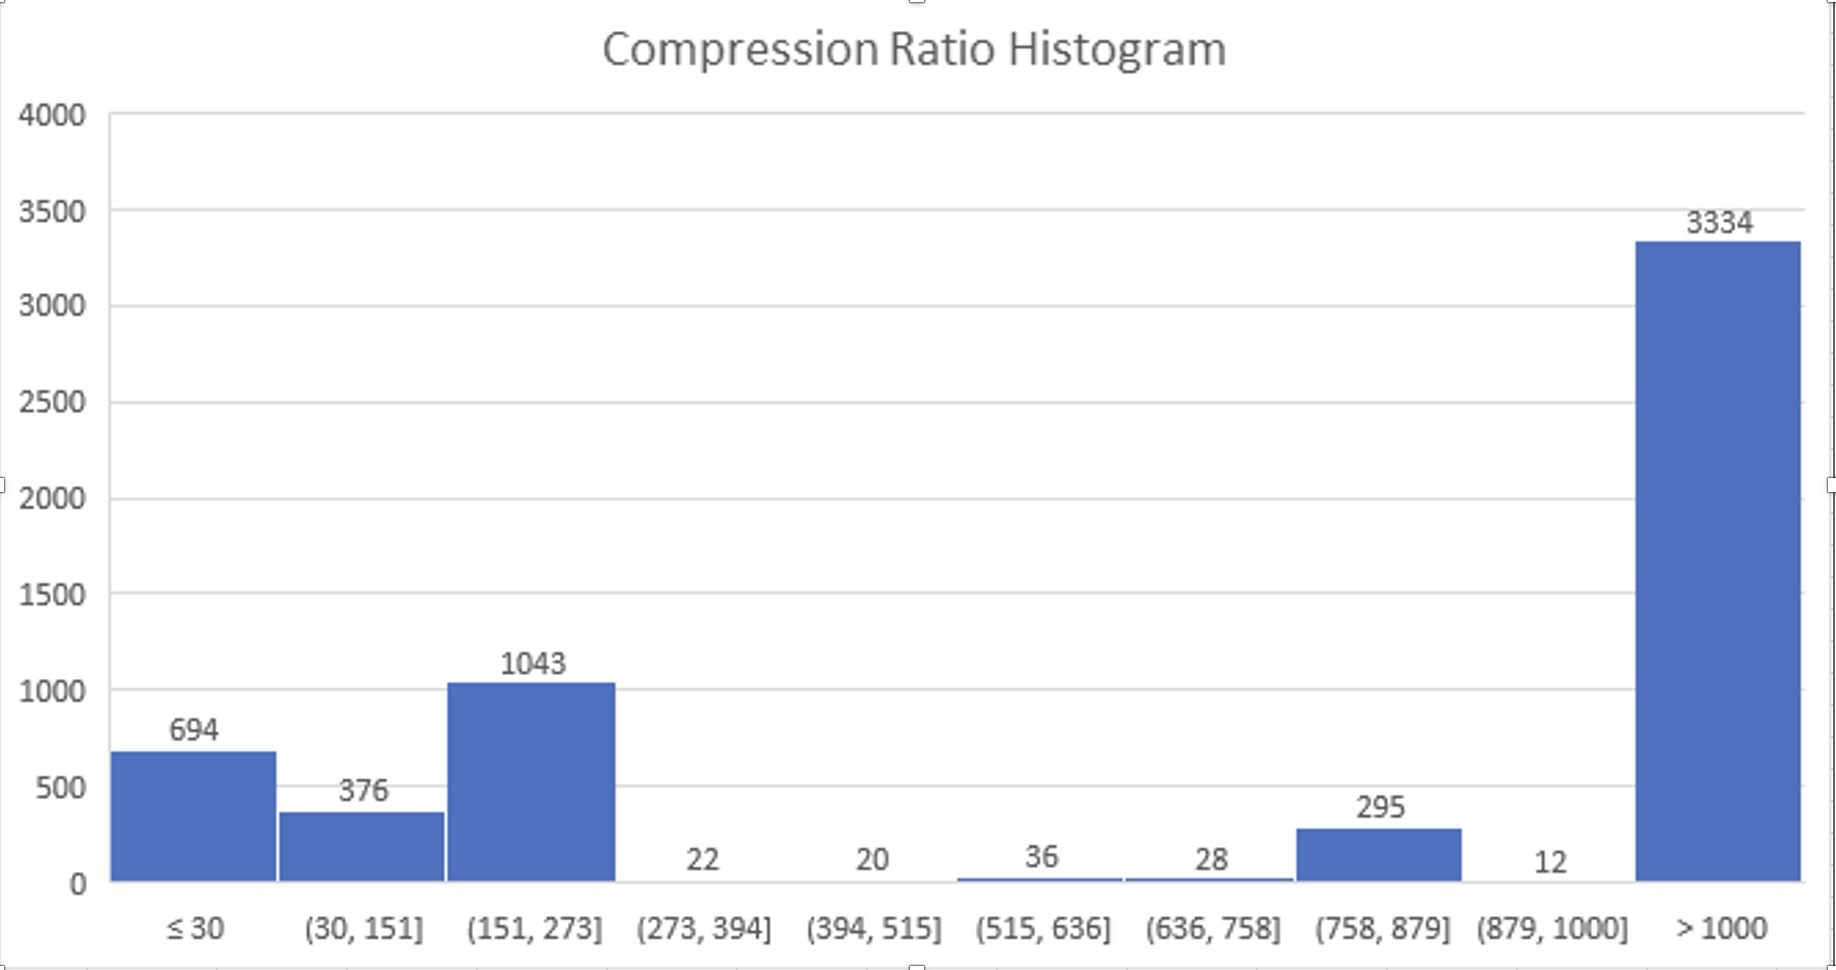
\includegraphics[width=0.5\textwidth]{Fig5.png}
  \caption{Compression Ratio Histogram}
  \label{Fig.6}
\end{figure}

\vspace{10pt}

These results offer a detailed insight into the performance of ATSC across various compression techniques. 
The data overview provides the baseline, while compression statistics and signal count shed light on the efficiency of ATSC's compression strategies. 
The analysis of compression ratios average and the histogram of compression further quantifies the compression effectiveness across the tested scenario. 
 
\subsection{Result validation}

For validation of the results, the data was uncompressed and compare with the original signal and see how was the fitting. Since the compressor was set to auto with an allowed error, the expectation is that there the compressor will pick lossy compression for best compression and that is visible in the fitting of the compressed signal vs the original data.

In this section we are going to show some examples of those compressed signals.

\begin{figure}[h]
  \centering
  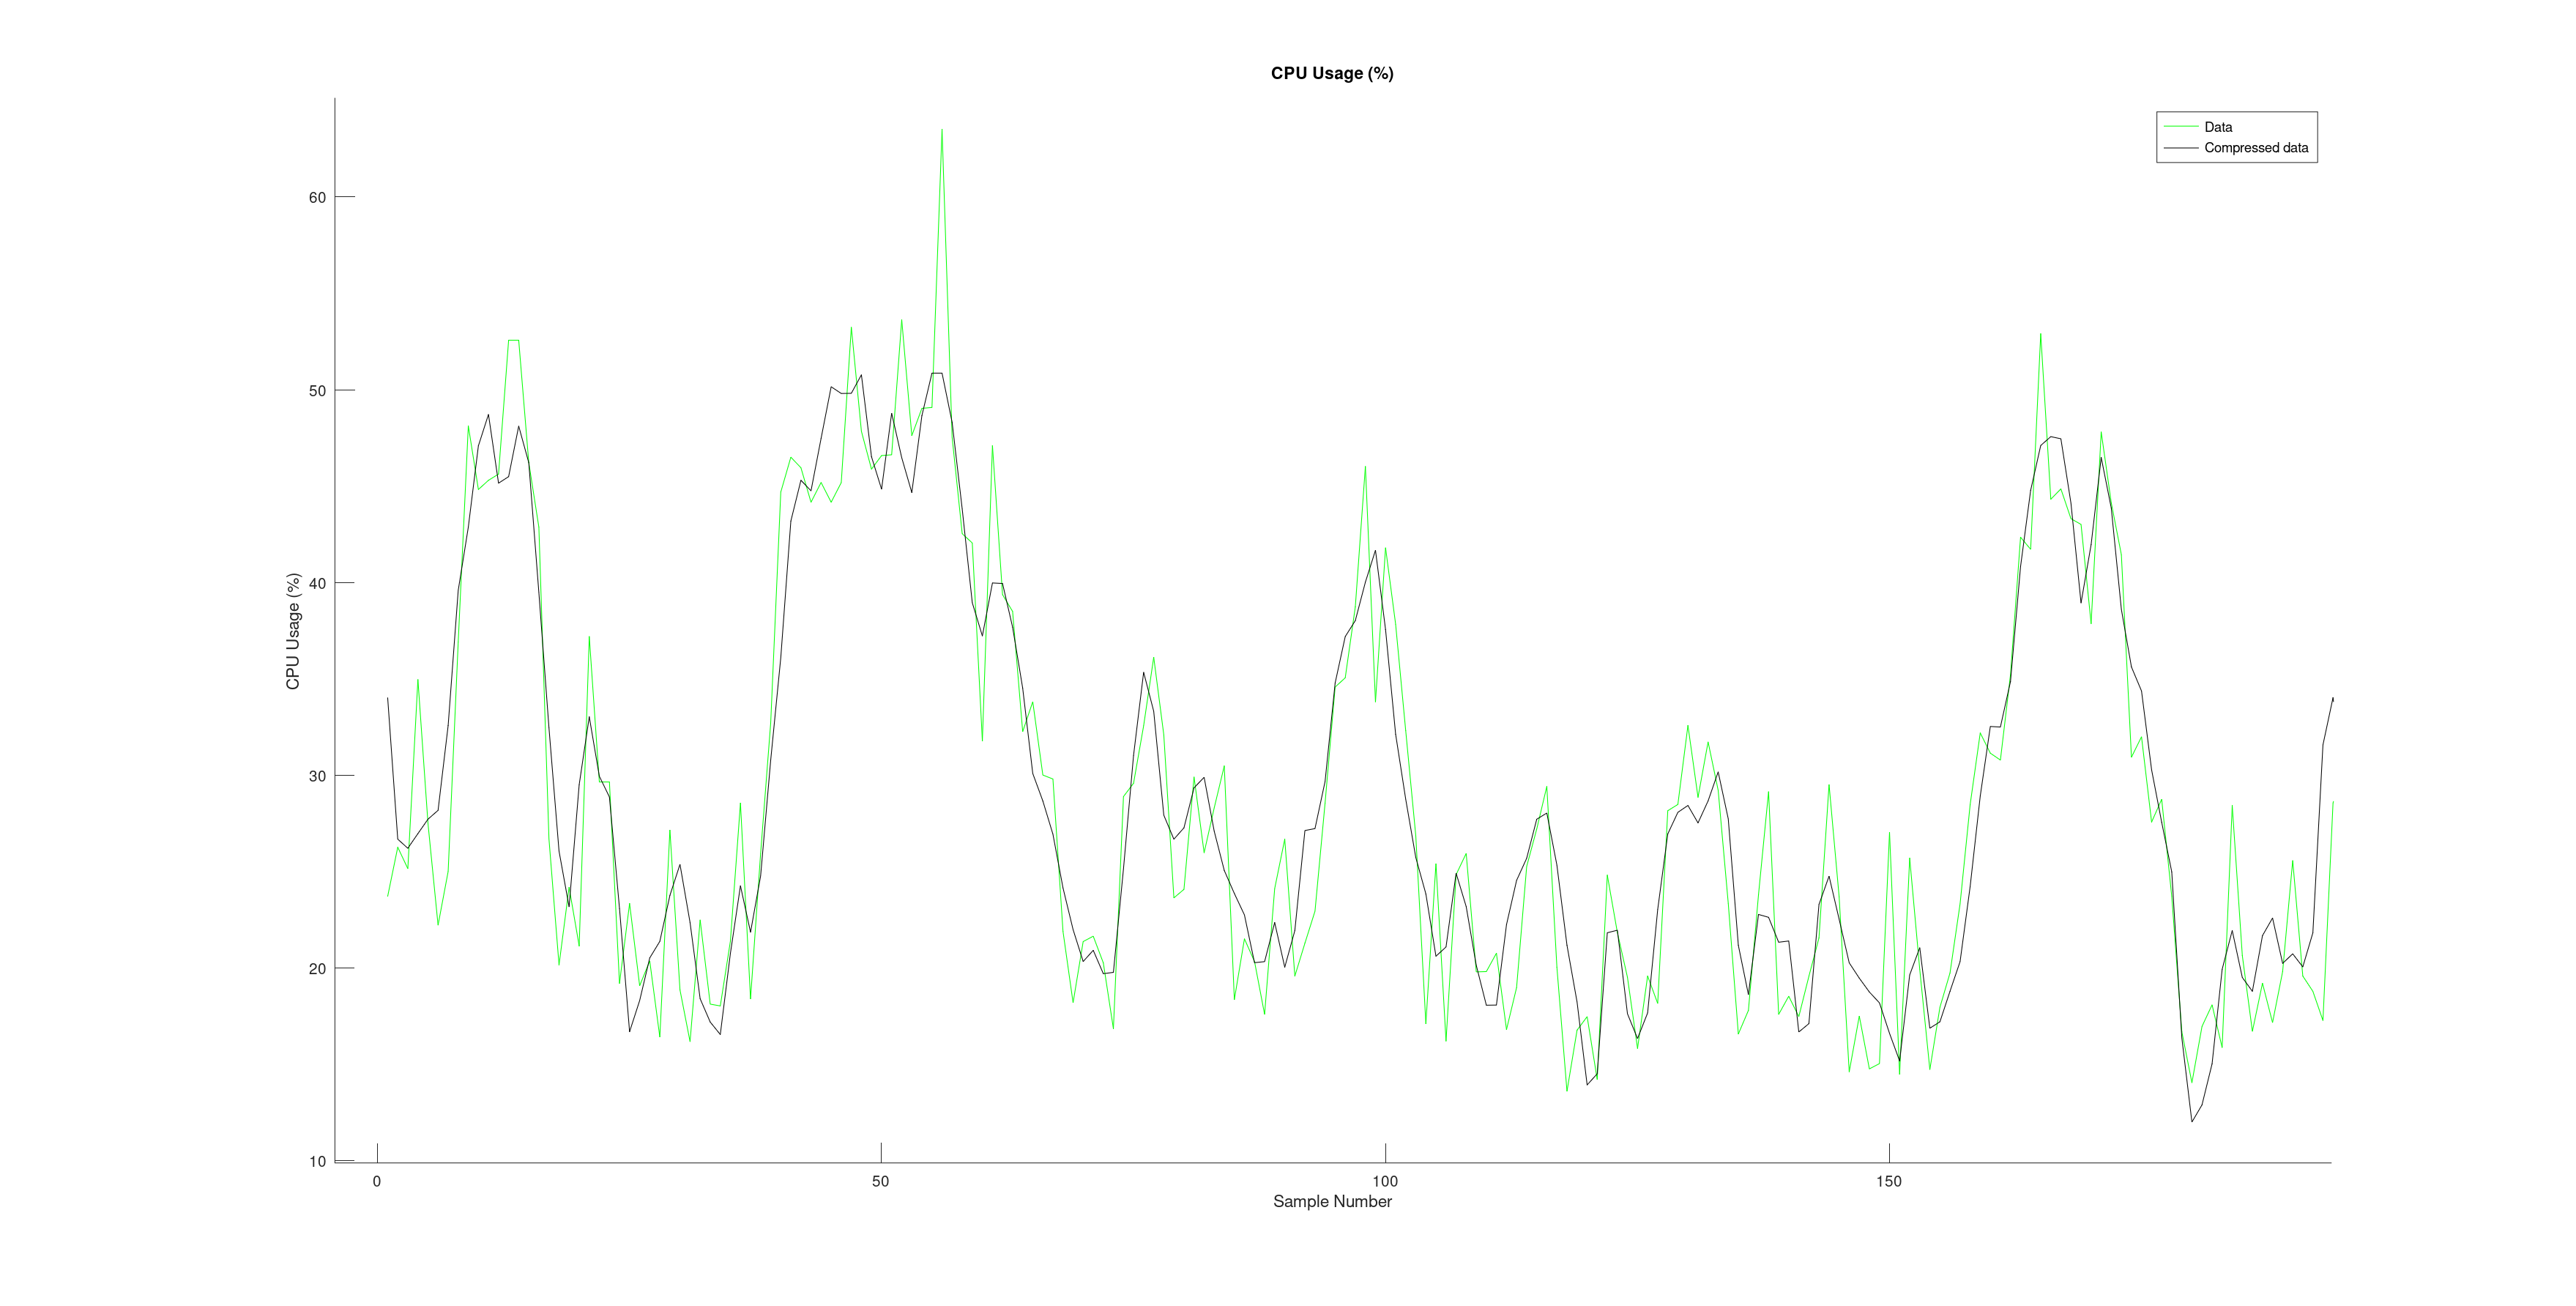
\includegraphics[width=0.5\textwidth]{cpu-usage-validation.png}
  \caption{CPU compression (17x) vs Original data}
  \label{cpu}
\end{figure}

We start with the CPU usage, this is signal that is always collected. 
The approximation is very close in the majority of the samples. 

\begin{figure}[h]
    \centering
    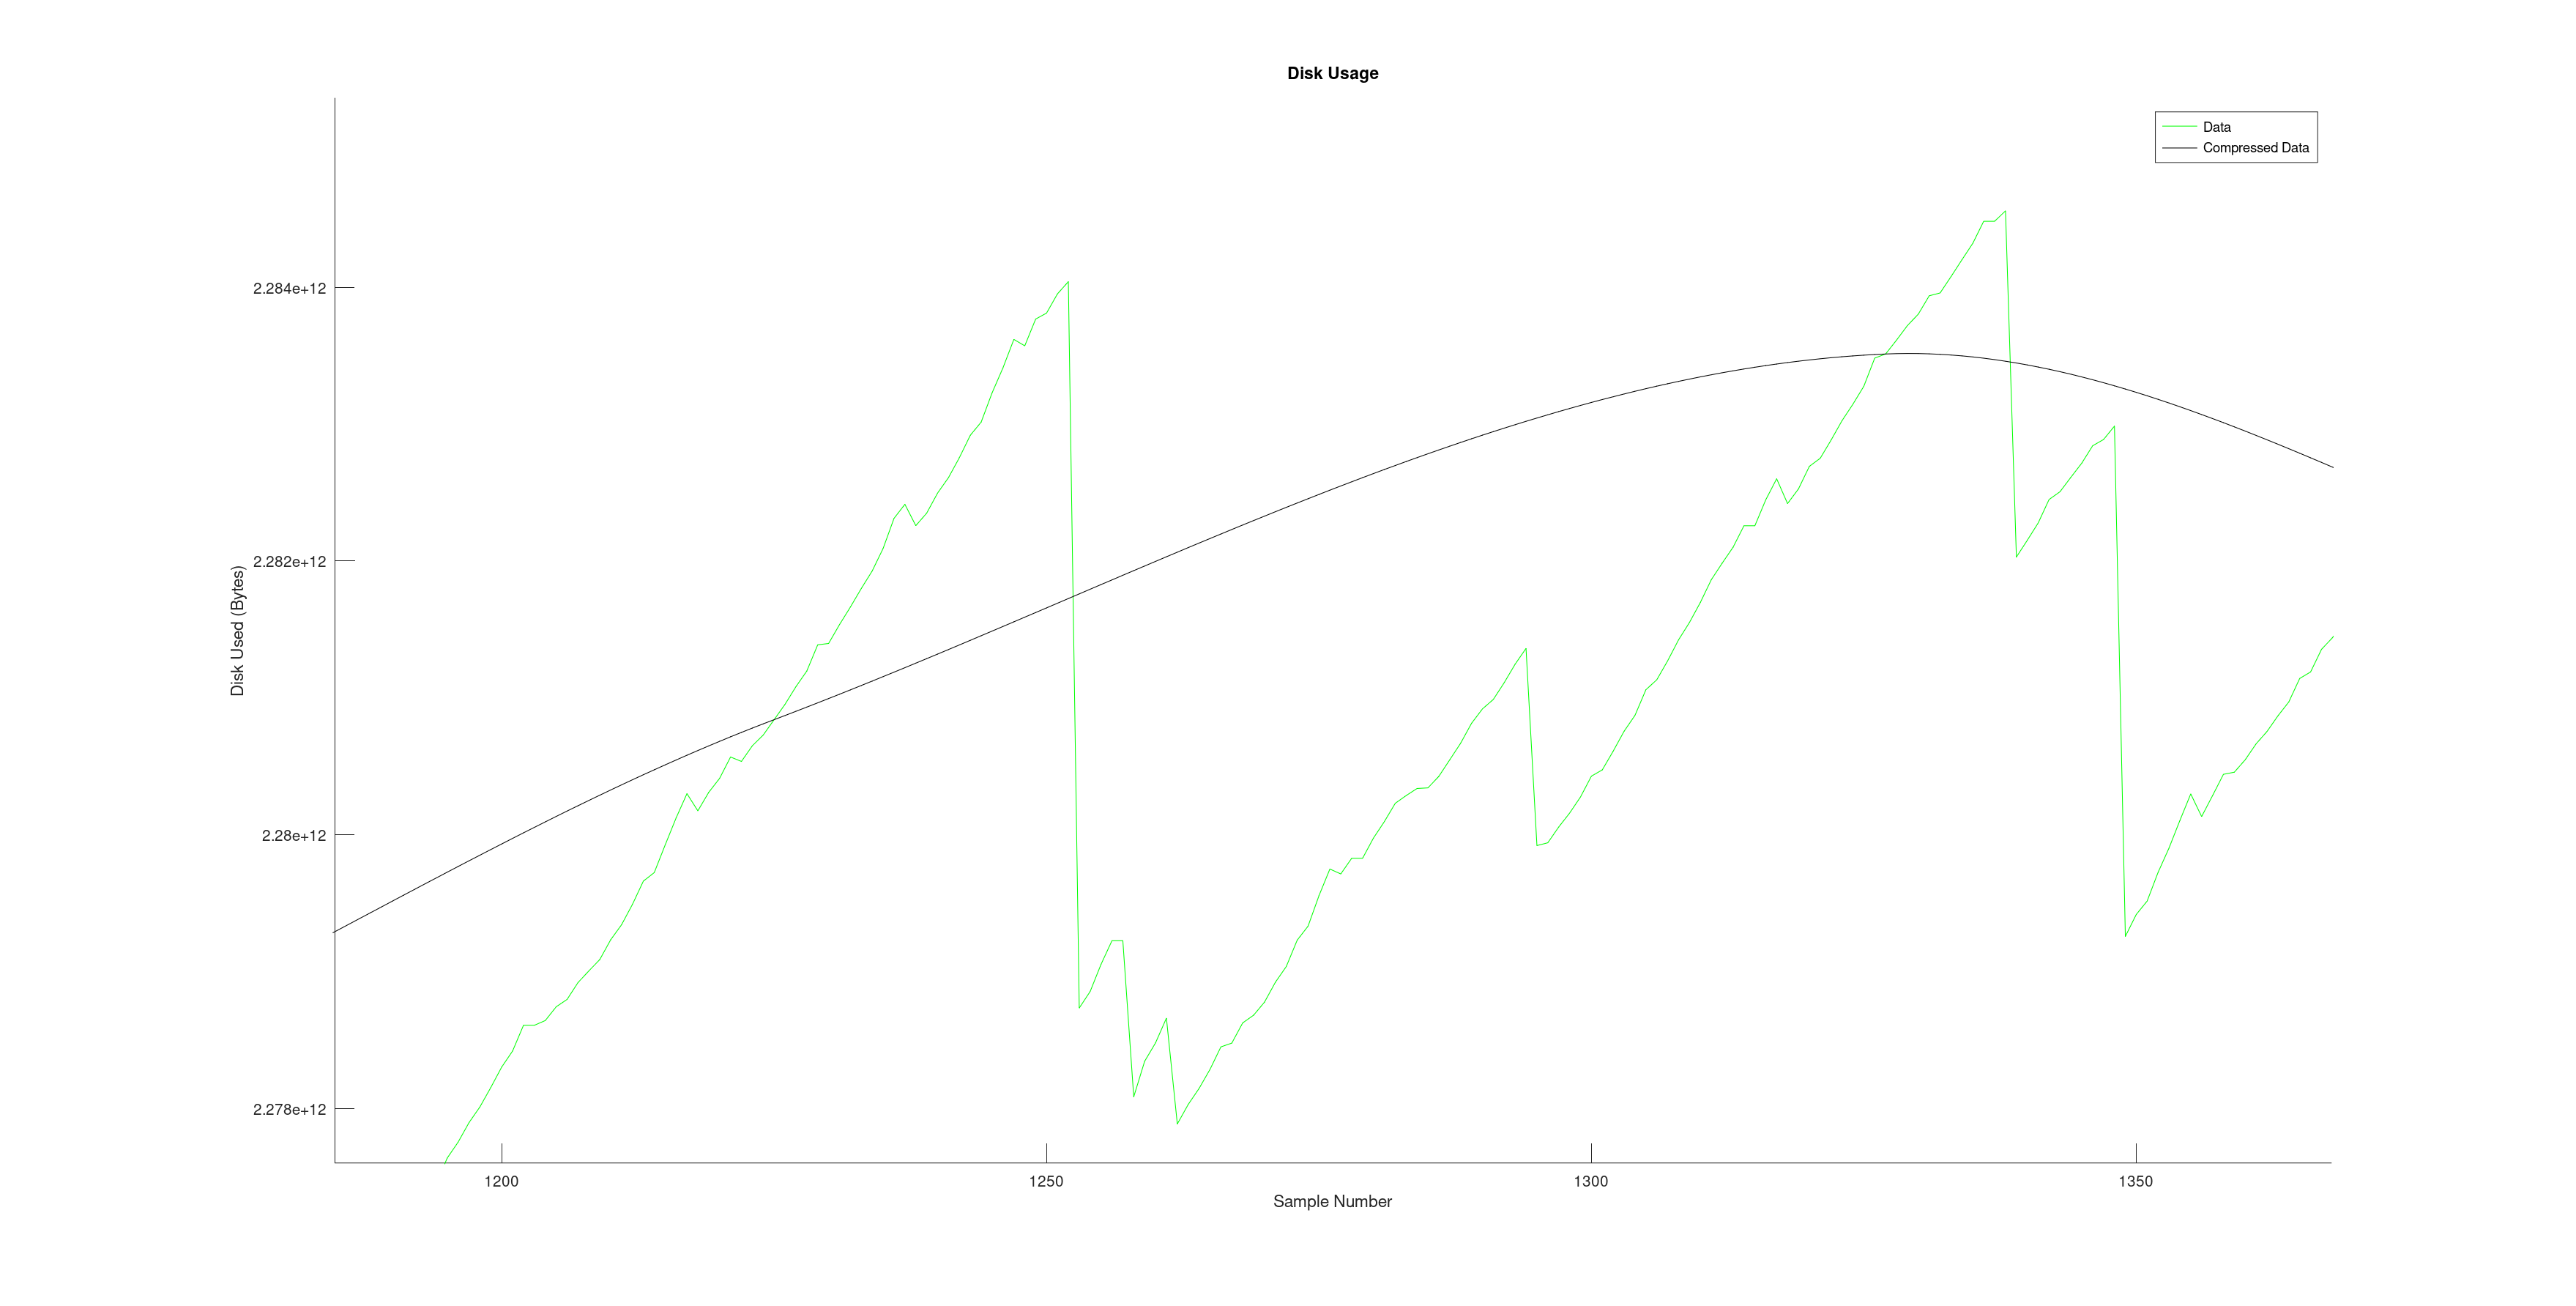
\includegraphics[width=0.5\textwidth]{disk-usage-validation.png}
    \caption{Disk compression (146x) vs Original data}
    \label{Disk}
  \end{figure}

Disk usage is another metric that is stored all the time.
And this signal show what could be a somewhat very wrong approximation.
But by looking at the scale, we can clearly see that the approximation does a description of the disk usage with less than 3\% error.

  \begin{figure}[h]
    \centering
    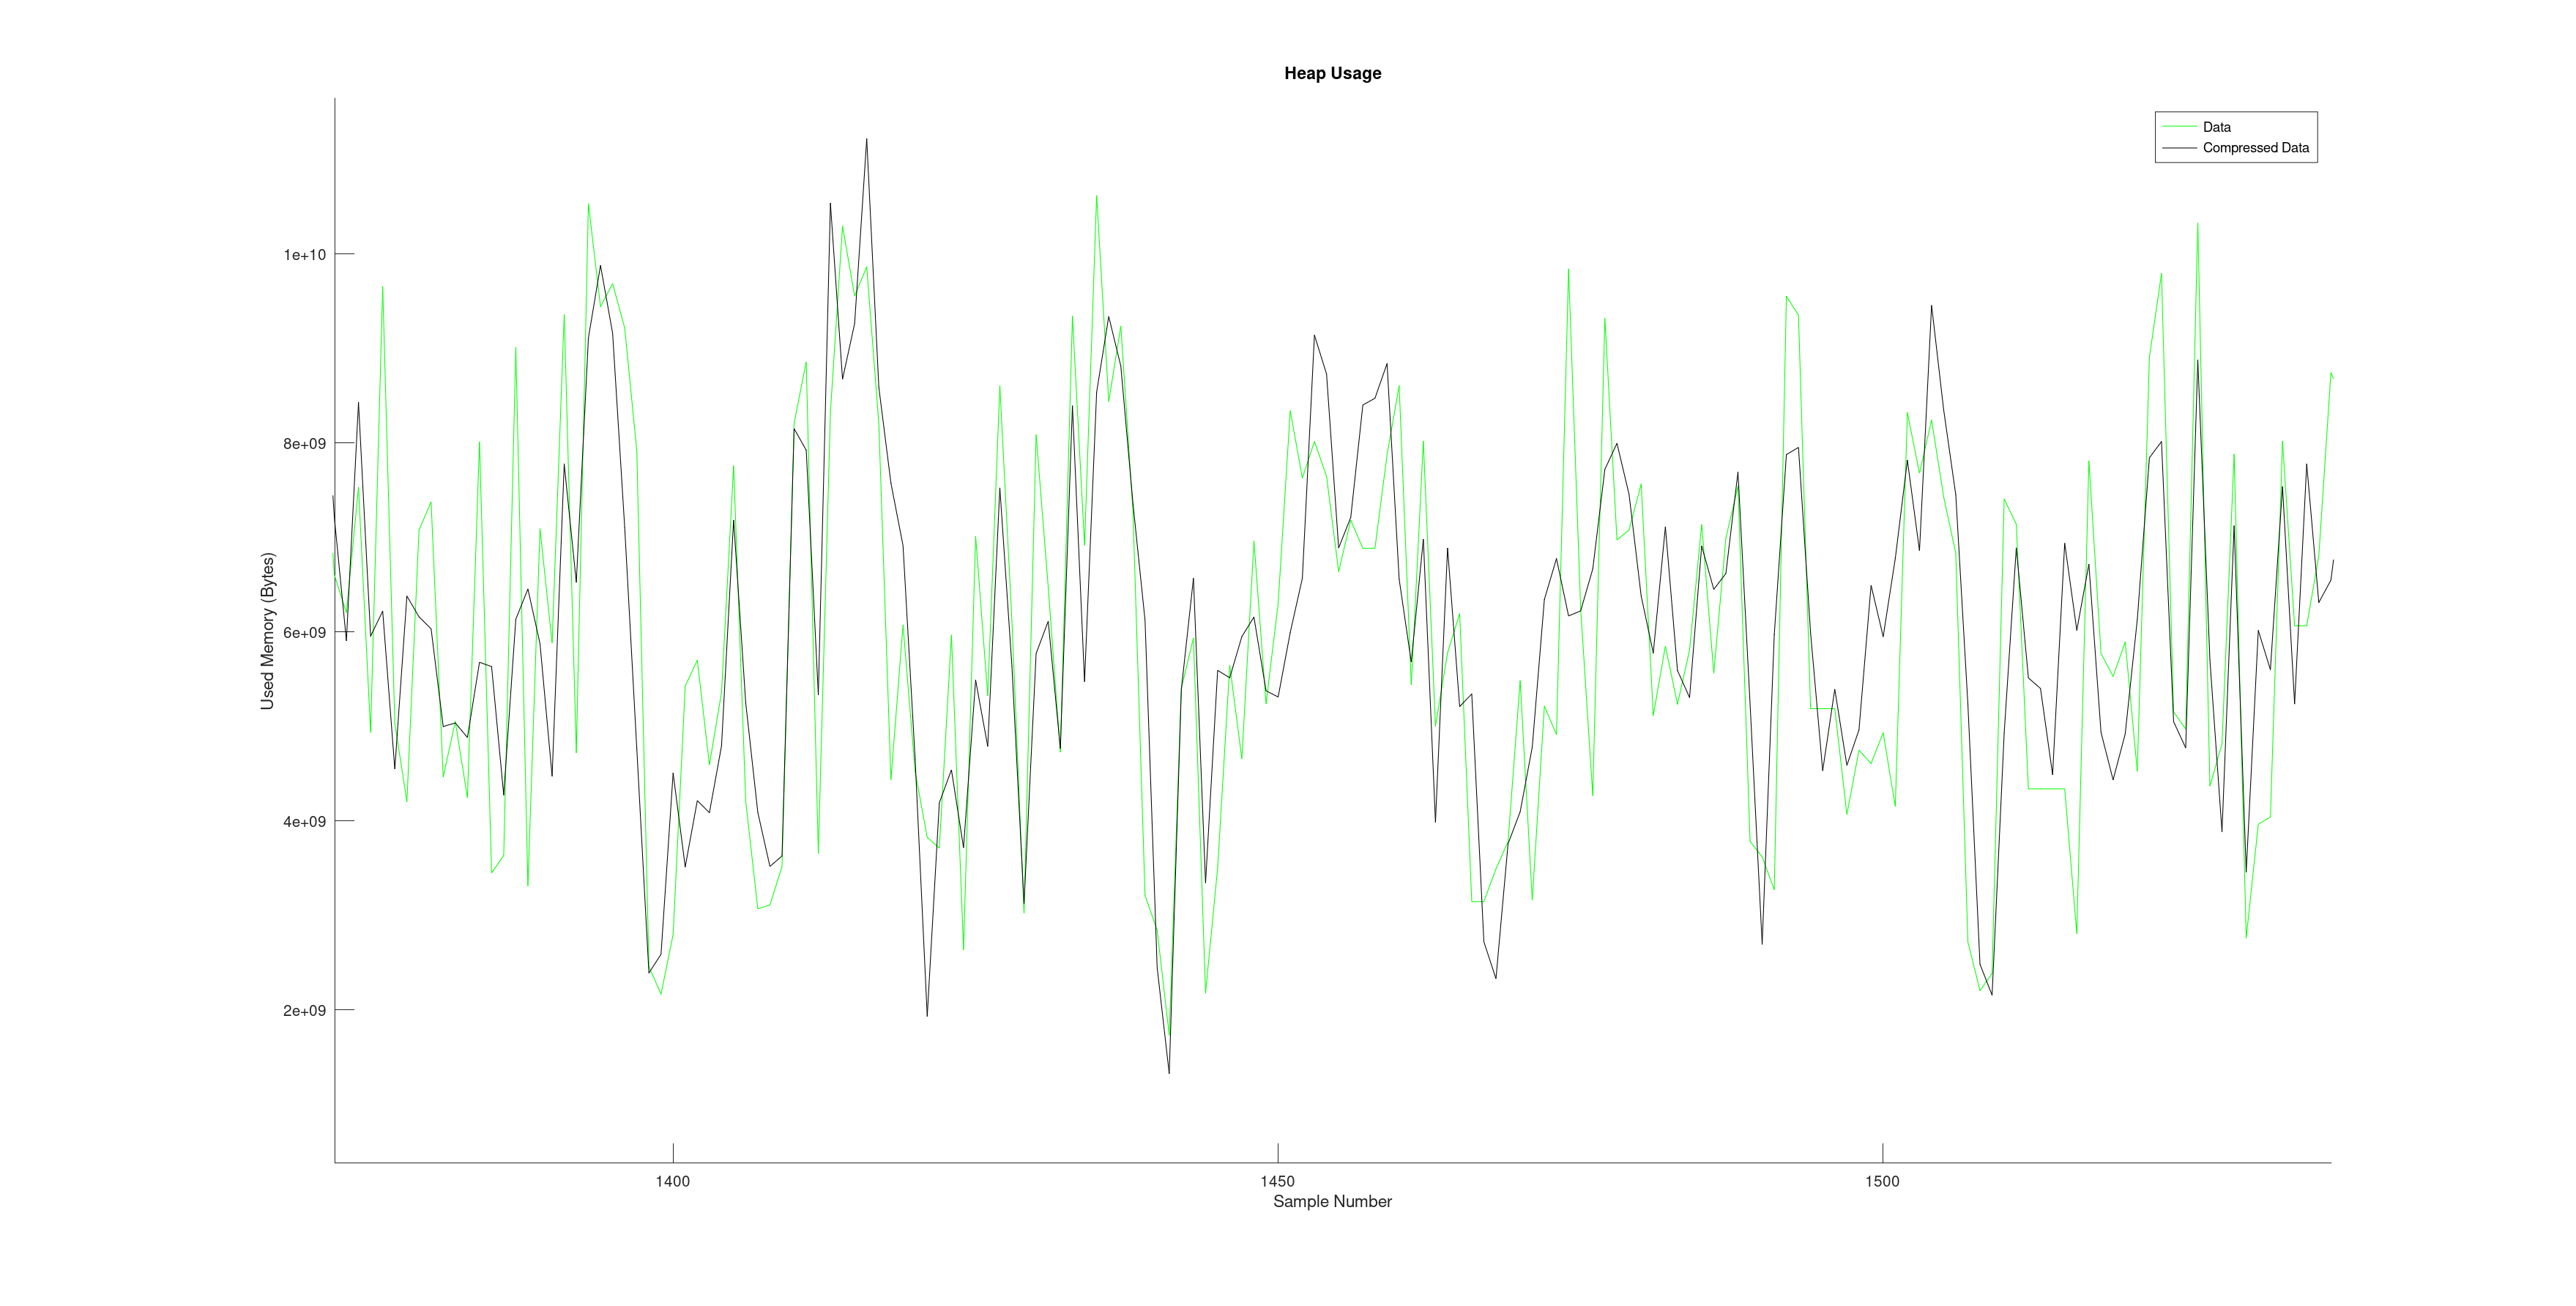
\includegraphics[width=0.5\textwidth]{heap-usage-validation.png}
    \caption{Heap Usage Compressed (18x) vs Original data}
    \label{heap}
  \end{figure}
\vspace{10pt}

Heap usage was picked because it is normally a very difficult signal to fit. But our approach tracks the signal with enough accuracy to capture the information. 
As stated before, a reduction with compression could lead to a better approximation, but our review with real data shows that it wasn't significant.

In conclusion, ATSC Compression exhibited an impressive compression ratio of 57.34 times, showcasing the potential of ATSC in achieving substantial data reduction. 
These results substantiate ATSC's capabilities in optimizing storage space, offering valuable insights into its potential impact on real-world applications. 

\section{Future Work}

ATSC show a significant improvement over existing compression for time-series. But there are several avenues of possible work to further expand its capabilities and/or use some of the opportunities it exposes.

\subsection{AI for compressor selection and optimization}

Currently, ATSC has a small subset of fixed algorithms available to chose from. The choice is made based on a simplistic statistical analysis. With a growing number of signals analyzed it could be possible to use AI to make an optimal choice. 
Also, AI could be used to make a more curated choice of algorithms available for compression.

\subsection*{Test further algorithms}

ATSC algorithm selection could be expanded alongside improved selection methods, that could further increase ATSC compression ratio.

\subsection{Integration with other systems}

While developing and researching we found that ATSC creates similar outputs for a lot of signals. Compression of a signal at a time doesn't allow us to benefit from this. By using ATSC integrated in a database/filesystem/etc. it would be possible
to identify such scenarios and avoid storing further once we know a particular output exists already, thus further increase space savings.

\subsection{Outlier detection}

One characteristic that was noted during result analysis, as that for systems with a lot of nodes doing the same work (e.g. Cassandra database with multiple nodes), compression ratios for a given metric across all nodes would be mostly the same.
In a couple of cases we found that some nodes had significant differences for some metrics (more than double, sometimes 10x worse compression). By looking into the detailed metrics we could find that the node was misbehaving, and it should be fixed 
or replaced. This opens a front worth exploring that is comparing compression ratios for outlier detection.

\subsection{Use of hardware capacities}

Our approach doesn't only yield savings in at-rest scenarios but also in transit and during compute processing.
By having the ability to leverage client-side devices [9], we enable efficient processing and transport of monitoring data. 
Integration in system-on-a-Chip architectures [8] could lead to further performance enhancements. 
This strategy positions our methodology at the forefront of efficient and resource-conscious computer systems monitoring.

\section{Conclusion}

In conclusion, the ATSC approach outlined in this research offers a novel solution for monitoring time series data compression, particularly in computer systems. By using a new approach, ATSC achieves impressive compression ratios, with a best-case scenario reaching over 1000x times compression. This innovative methodology not only addresses current storage and data transfer challenges but also sets the stage for future improvements.
\vspace{5pt}
Preliminary testing against a Production cluster demonstrates significant space savings in the ATSC compared to currently state-of-the-art methods. The research emphasizes the importance of unique indexing for precise data retrieval, showcasing its efficiency in streaming and targeted decompression of relevant data segments.

The outlined future work underscores ATSC's commitment to continuous improvement, with a focus on automated selections, integration with time series databases, and adding other capabilities. These efforts aim to keep ATSC at the forefront of efficient and intelligent time series data compression.

In summary, ATSC emerges as a promising solution that not only tackles current challenges but also paves the way for ongoing advancements in the dynamic landscape of time series data compression.

\bibliographystyle{plain} % We choose the "plain" reference style
\bibliography{refs} % Entries are in the refs.bib file
\end{document}